\subsection{Introduction. Gravitational waves, probe of the early universe}

Como consecuencia de que la gravedad no es muy fuerte, las ondas gravitatorias se encuentran desacopladas del resto de componentes del universo (materia y radiación). Ésto lo podemos viendo teniendo en cuenta que la tasa de interacción es $\Gamma = n \sigma v$, entonces para las ondas gravitatorias tenemos $v \simeq 1$, $n \sim T^3$ y $\sigma \sim G^2 T^2$ y el parámetro de Hubble de las ecuaciones de Friedmann podemos ver que va como $\displaystyle H \sim \frac{T^2}{M_{pl}}$, siendo $M_{pl} = G^{-1/2}$ la masa de Planck. De este modo, podemos ver que para $T < M_{pl}$ tenemos que $\Gamma < H$ lo que implica que las ondas gravitatorias se propagan libremente en el universo llevando consigo la información de la producción de éstas, por tanto la información sobre el estado del universo en aquel momento.

\subsection{Definition of gravitational waves}

\subsubsection{Linearized theory in vacuum: the transverse-treceless gauge}

Uno puede definir a las ondas gravitacionales a partir de una perturbación pequeña en la métrica. De forma tal que la métrica para una métrica de fondo $\eta_{\mu\nu}$, se escribe como

\begin{equation}
    g_{\mu \nu} = \eta_{\mu\nu} + h_{\mu\nu}
\end{equation}

\noindent
dónde $\left| h_{\mu\nu} \right| \ll 1$, y la métrica de fondo $\eta_{\mu\nu}$ es generalmente la métrica de Minkowski.

Sabiendo que la física no puede depender del sistema de coordenadas elegido podemos plantear que ante un cambio de coordenadas de la forma $x'^{\mu} = x^\mu + \xi^\mu$, la métrica cambia como

\begin{equation}
    g_{\mu\nu} (x) = \frac{\partial x'^\alpha}{\partial x^\mu} \frac{\partial x'^\beta}{\partial x^\nu} g'_{\alpha\beta} (x')
\end{equation}

\begin{equation}
    \begin{split}
        g_{\mu\nu} (x) &= \partial_\mu \left( x^\alpha + \xi^\alpha \right) \ \partial_\nu \left( x^\beta + \xi^\beta \right) \ \left[ \eta_{\alpha \beta} + h'_{\alpha \beta} (x') \right]\\
        &= \left( \delta^\alpha_\mu + \partial_\mu \xi^\alpha \right) \left( \delta^\beta_\nu + \partial_\nu \xi^\beta \right) \left[ \eta_{\alpha \beta} + h'_{\alpha \beta} (x') \right]\\
        &= \left( \delta^\alpha_\mu + \partial_\mu \xi^\alpha \right) \left[ \delta^\beta_\nu \eta_{\alpha \beta} + \left( \partial_\nu \xi^\beta \right) \eta_{\alpha \beta} + \delta^\beta_\nu h'_{\alpha \beta} (x') + \left( \partial_\nu \xi^\beta \right) h'_{\alpha \beta} (x') \right]\\
        &= \left( \delta^\alpha_\mu + \partial_\mu \xi^\alpha \right) \left[ \eta_{\alpha \nu} + \partial_\nu \xi_\alpha + h'_{\alpha \nu} (x') + \left( \partial_\nu \xi^\beta \right) h'_{\alpha \beta} (x') \right]
    \end{split}
\end{equation}

\noindent
como $\left| h_{\alpha \beta} \right| \ll 1$ y $\xi^\mu \ll 1$, entonces podemos tirar los términos de orden cuadrático

\begin{equation}
    \begin{split}
        g_{\mu\nu} (x) &\simeq \left( \delta^\alpha_\mu + \partial_\mu \xi^\alpha \right) \left[ \eta_{\alpha \nu} + \partial_\nu \xi_\alpha + h'_{\alpha \nu} (x') \right]\\
        \eta_{\mu\nu} + h_{\mu\nu} (x) &\simeq \delta^\alpha_\mu \eta_{\alpha \nu} + \left( \partial_\mu \xi^\alpha \right) \eta_{\alpha \nu} + \delta^\alpha_\mu \partial_\nu \xi_\alpha + \left( \partial_\mu \xi^\alpha \right) \left( \partial_\nu \xi_\alpha \right) + \delta_\mu^\alpha h'_{\alpha \nu} (x') + \left( \partial_\mu \xi^\alpha \right) h'_{\alpha \nu} (x')\\
        \eta_{\mu \nu} + h_{\mu \nu} (x) &\simeq \eta_{\mu \nu} + \partial_\mu \xi_\nu + \partial_\nu \xi_\mu + h'_{\mu \nu} (x') 
    \end{split}
\end{equation}

\begin{equation}
    h'_{\mu \nu} (x') = h_{\mu \nu} (x) - \partial_\mu \xi_\nu - \partial_\nu \xi_\mu 
\end{equation}

\noindent
ésto significa que la métrica tiene una simetría de gauge dada por el parámetro $\xi^\mu$.

Por otro lado, tenemos que la métrica definida nos da los siguientes símbolos de Christoffel

\begin{equation}
    \Gamma^\mu_{\alpha \beta} = \frac{g^{\mu \nu}}{2} \left( \partial_\beta g_{\alpha \nu} + \partial_\alpha g_{\beta \nu} - \partial_\nu g_{\alpha \beta} \right)
\end{equation}

\begin{equation}
    \begin{split}
        \Gamma^\mu_{\alpha \beta} &= \frac{1}{2} \left( \eta^{\mu \nu} + h^{\mu \nu} \right) \left[ \partial_\beta \left( \eta_{\alpha \nu} + h_{\alpha \nu} \right) + \partial_\alpha \left( \eta_{\beta \nu} + h_{\beta \nu} \right) - \partial_\nu \left( \eta_{\alpha \beta} + h_{\alpha \beta} \right) \right]\\
        &= \frac{1}{2} \left( \eta^{\mu \nu} + h^{\mu \nu} \right) \left( \partial_\beta h_{\alpha \nu} + \partial_\alpha h_{\beta \nu} - \partial_\nu h_{\alpha \beta} \right)\\
        &\simeq \frac{\eta^{\mu \nu}}{2} \left( \partial_\beta h_{\alpha \nu} + \partial_\alpha h_{\beta \nu} - \partial_\nu h_{\alpha \beta} \right)\\
        \Gamma^\mu_{\alpha \beta} &\simeq \frac{1}{2} \left( \partial_\beta h_\alpha^\mu + \partial_\alpha h_\beta^\mu - \partial^\mu h_{\alpha \beta}  \right)
    \end{split}
\end{equation}

\noindent
con los símbolos de Christoffel podemos calcular el tensor de Riemann, el tensor de Ricci y el escalar de Ricci

\begin{equation}
    \begin{split}
        R^\beta_{\mu \nu \alpha} &= \partial_\nu \Gamma^\beta_{\mu \alpha} - \partial_\mu \Gamma^\beta_{\nu \alpha} + \overbrace{\Gamma_{\mu \alpha}^\sigma \Gamma_{\sigma \nu}^\beta - \Gamma_{\nu \alpha}^\sigma \Gamma^\beta_{\sigma \mu}}^{\mathcal{O}(h^2)}\\
        &\simeq \frac{\partial_\nu}{2} \left( \partial_\alpha h_\mu^\beta + \partial_\mu h^\beta_\alpha - \partial^\beta h_{\mu \alpha}  \right) - \frac{\partial_\mu}{2} \left( \partial_\alpha h_\nu^\beta + \partial_\nu h^\beta_\alpha - \partial^\beta h_{\nu \alpha} \right)\\
        &\simeq \frac{1}{2} \left( \partial_\nu \partial_\alpha h_\mu^\beta \textcolor{red}{+ \partial_\nu \partial_\mu h^\beta_\alpha} - \partial_\nu \partial^\beta h_{\mu \alpha} - \partial_\mu \partial_\alpha h_\nu^\beta \textcolor{red}{- \partial_\mu \partial_\nu h_\alpha^\beta} + \partial_\mu \partial^\beta h_{\nu \alpha} \right)\\
        &\simeq \frac{1}{2} \left( \partial_\nu \partial_\alpha h_\mu^\beta - \partial_\nu \partial^\beta h_{\mu \alpha} - \partial_\mu \partial_\alpha h_\nu^\beta + \partial_\mu \partial^\beta h_{\nu \alpha} \right)
    \end{split}
\end{equation}

\begin{equation}
    \begin{split}
        R_{\mu\nu} &= R_{\mu \alpha \nu}^\alpha\\
        &= \frac{1}{2} \left( \partial_\alpha \partial_\nu h_\mu^\alpha - \partial_\alpha \partial^\alpha h_{\mu \nu} - \partial_\mu \partial_\nu h_\alpha^\alpha + \partial_\mu \partial^\alpha h_{\alpha \nu} \right)\\
        &= \frac{1}{2} \left( \partial_\nu \partial^\alpha h_{\alpha \mu} - \Box h_{\mu \nu} - \partial_\mu \partial_\nu h + \partial_\mu \partial^\alpha h_{\alpha \nu} \right)
    \end{split}
\end{equation}

\begin{equation}
    \begin{split}
        R &= g^{\mu \nu} R_{\mu \nu}\\
        &= \frac{1}{2} \left( \eta^{\mu \nu} + h^{\mu \nu} \right) \left( \partial_\nu \partial^\alpha h_{\alpha \mu} - \Box h_{\mu \nu} - \partial_\mu \partial_\nu h + \partial_\mu \partial^\alpha h_{\alpha \nu} \right)\\
        &\simeq \frac{\eta^{\mu \nu}}{2} \left( \partial_\nu \partial^\alpha h_{\alpha \mu} - \Box h_{\mu \nu} - \partial_\mu \partial_\nu h + \partial_\mu \partial^\alpha h_{\alpha \nu} \right)\\
        &= \frac{1}{2} \left( \partial^\mu \partial^\alpha h_{\alpha \mu} - \Box h - \Box h + \partial^\nu \partial^\alpha h_{\alpha \nu} \right)\\
        &= \partial^\mu \partial^\nu h_{\mu \nu} - \Box h
    \end{split} 
\end{equation}

\noindent
a su vez, con ésto, podemos calcular el tensor de Einstein, definiendo $\displaystyle \bar{h}_{\mu \nu} = h_{\mu \nu} - \frac{1}{2} \eta_{\mu \nu} h$ por lo que $\bar{h} = - h$

\begin{equation}
    \begin{split}
        G_{\mu \nu} &= R_{\mu \nu} - \frac{1}{2} g_{\mu \nu} R\\
        &= \frac{1}{2} \left( \partial_\nu \partial^\alpha h_{\alpha \mu} - \Box h_{\mu \nu} - \partial_\mu \partial_\nu h + \partial_\mu \partial^\alpha h_{\alpha \nu} \right) - \frac{1}{2} \left( \eta_{\mu \nu} + h_{\mu \nu} \right) \left( \partial^\alpha \partial^\beta h_{\alpha \beta} - \Box h \right)\\
        &\simeq \frac{1}{2} \left( \partial_\nu \partial^\alpha h_{\alpha \mu} - \Box h_{\mu \nu} - \partial_\mu \partial_\nu h + \partial_\mu \partial^\alpha h_{\alpha \nu} \right) - \frac{\eta_{\mu \nu}}{2} \left( \partial^\alpha \partial^\beta h_{\alpha \beta} - \Box h \right)\\
        &= \frac{1}{2} \left( \partial_\nu \partial^\alpha h_{\alpha \mu} - \Box h_{\mu \nu} -\partial_\mu \partial_\nu h + \partial_\mu \partial^\alpha h_{\alpha \nu} - \eta_{\mu \nu} \partial^\alpha \partial^\beta h_{\alpha \beta} + \eta_{\mu \nu} \Box h \right)\\
        &= \frac{1}{2} \left[ \partial_\nu \partial^\alpha h_{\alpha \mu} - \eta_{\alpha \mu} \partial_\nu \partial^\alpha h - \Box \left( h_{\mu \nu} - \frac{1}{2} \eta_{\mu \nu} h \right) + \frac{1}{2} \eta_{\mu \nu} \Box h + \partial_\mu \partial^\alpha h_{\alpha \nu} - \eta_{\mu \nu} \partial^\alpha \partial^\beta h_{\alpha \beta} \right]\\
        &= \frac{1}{2} \left[ \partial_\nu \partial^\alpha \left( h_{\alpha \mu} - \frac{1}{2} \eta_{\alpha \mu} h \right) - \Box \bar{h}_{\mu \nu} - \frac{1}{2} \eta_{\alpha \mu} \partial^\alpha \partial_\nu h + \frac{1}{2} \eta_{\mu \nu} \partial^\alpha \partial_\alpha h + \partial_\mu \partial^\alpha h_{\alpha \nu} - \eta_{\mu \nu} \partial^\alpha \partial^\beta h_{\alpha \beta} \right]\\
        &= \frac{1}{2} \left[ \partial_\nu \partial^\alpha \bar{h}_{\alpha \mu} - \Box \bar{h}_{\mu \nu} - \frac{1}{2} \partial_\mu \partial_\nu h + \partial_\mu \partial^\alpha h_{\alpha \nu} - \eta_{\mu \nu} \partial^\alpha \left( \partial^\beta h_{\alpha \beta} - \frac{1}{2} \partial_\alpha h \right) \right]\\
        &= \frac{1}{2} \left[ \partial_\nu \partial^\alpha \bar{h}_{\alpha \mu} - \Box \bar{h}_{\mu \nu} + \partial_\mu \left(\partial^\alpha h_{\alpha \nu} - \frac{1}{2} \partial_\nu h \right) - \eta_{\mu \nu} \partial^\alpha \left( \partial^\beta h_{\alpha \beta} - \frac{1}{2} \eta_{\alpha \beta} \partial^\beta h \right) \right]\\
        &= \frac{1}{2} \left[ \partial_\nu \partial^\alpha \bar{h}_{\alpha \mu} - \Box \bar{h}_{\mu \nu} + \partial_\mu \left( \partial^\alpha h_{\alpha \nu} - \frac{1}{2} \eta_{\nu \alpha} \partial^\alpha h \right) - \eta_{\mu \nu} \partial^\alpha \partial^\beta \left( h_{\alpha \beta} - \frac{1}{2} \eta_{\alpha \beta} h \right) \right]\\
        &= \frac{1}{2} \left[ \partial_\nu \partial^\alpha \bar{h}_{\alpha \mu} - \Box \bar{h}_{\mu \nu} + \partial_\mu \partial^\alpha \left( h_{\alpha \nu} - \frac{1}{2} \eta_{\nu \alpha} h \right) - \eta_{\mu \nu} \partial^\alpha \partial^\beta \bar{h}_{\alpha \beta} \right]\\
        &= \frac{1}{2} \left( \partial_\nu \partial^\alpha \bar{h}_{\alpha \mu} - \Box \bar{h}_{\mu \nu} + \partial_\mu \partial^\alpha \bar{h}_{\alpha \nu} - \eta_{\mu \nu} \partial^\alpha \partial^\beta \bar{h}_{\alpha \beta} \right)
    \end{split}
\end{equation}

\noindent
el escribir el tensor de Einstein en términos de $\bar{h}$, nos permite eliminar la traza de este tensor. A su vez, podemos definir al gauge de Lorentz como

\begin{equation}
    \partial^\mu \bar{h}_{\mu \nu} = 0
\end{equation}

\noindent
lo que nos deja con que en este gauge el tensor de Einstein se escribe como

\begin{equation}
    G_{\mu\nu} = - \frac{1}{2} \Box \bar{h}_{\mu \nu}
\end{equation}

A partir de todo lo mencionado podemos escribir la ecuación de ondas usando la ecuación de Einstein como

\begin{equation}
    G_{\mu \nu} = \frac{1}{m_p^2} T_{\mu \nu} \Rightarrow \boxed{\Box \bar{h}_{\mu \nu} = - \frac{2}{m_p^2} T_{\mu \nu}}
\end{equation}

La solución a la ecuación de onda homogénea es de la forma

\begin{equation}
    \bar{h}_{\mu \nu} (x) = \int \left[ \bar{h}_{\mu \nu} (\textbf{k}) \ e^{ikx} + \bar{h}^*_{\mu \nu} (\textbf{k}) \ e^{-ikx} \right] \ d^3 k
\end{equation}

\noindent
dónde $kx = k^\mu x_\mu = - \omega t + \textbf{k} \cdot \textbf{x}$, $\omega = \left| \textbf{k} \right|$, y $k^\mu \bar{h}_{\mu \nu} = 0$. La última condición sale de usar el gauge de Lorentz.

Podemos sacarnos las libertades de gauge en la métrica al definir al gauge transverso y sin traza de la siguiente forma:

\begin{equation}
    h_{\mu 0} = 0 \hspace{2cm} h = 0
\end{equation}

\noindent
usar este gauge nos permite notar que $h_{\mu \nu} = \bar{h}_{\mu \nu}$. Con este gauge, definiendo la dirección de movimiento de la onda como $\hat{z}$ y usando que este tensor es simétrico, tenemos que se escribe como

\begin{equation}
    h_{\mu \nu} = \begin{pmatrix}
        0 & 0 & 0 & 0\\
        0 & h_+ & h_\times & 0\\
        0 & h_\times & - h_+ & 0\\
        0 & 0 & 0 & 0
    \end{pmatrix} = h_+ \begin{pmatrix}
        0 & 0 & 0 & 0\\
        0 & 1 & 0 & 0\\
        0 & 0 & -1 & 0\\
        0 & 0 & 0 & 0
    \end{pmatrix} + h_\times \begin{pmatrix}
        0 & 0 & 0 & 0\\
        0 & 0 & 1 & 0\\
        0 & 1 & 0 & 0\\
        0 & 0 & 0 & 0
    \end{pmatrix}
\end{equation}

\noindent
dónde $h_+$ y $h_\times$ son las dos polarizaciones posibles de las ondas gravitatorias. A partir de todo lo mencionado, también, podemos escribir a la métrica como

\begin{equation}
    ds^2 = - dt^2 + (1 + h_+) \ dx^2 + (1 - h_- ) \ dy^2 + 2 h_\times \ dx \ dy + dz^2
\end{equation}

\subsubsection{Linearized theory in matter: scalar-vector-tensor decomposition}

Acá todavía usaremos como métrica de fondo a la de Minkowski, pero separaremos a la perturbación de la métrica en componentes irreducibles frente a rotaciones espaciales. Esta separación la haremos de la siguiente forma: 

\begin{equation}
    \begin{cases}
        \displaystyle \delta g_{00} = - 2 \textcolor{blue}{\phi}\\
        \displaystyle \delta g_{i0} = \partial_i \textcolor{blue}{B} + \textcolor{green}{S_i} \\
        \displaystyle \delta g_{ij} = - 2 \textcolor{blue}{\psi} \ \delta_{ij} + \left( \partial_i \partial_j - \frac{\delta_{ij}}{3} \nabla^2 \right) \textcolor{blue}{E} + \partial_i \textcolor{green}{F}_j + \partial_j \textcolor{green}{F_i} + \textcolor{red}{h_{ij}}
    \end{cases}
\end{equation}

\noindent
y para el tensor de energía-impulso tenemos

\begin{equation}
    \begin{cases}
        \displaystyle T_{00} = \textcolor{blue}{\rho}\\
        \displaystyle T_{0i} = \partial_i \textcolor{blue}{u} + \textcolor{green}{u_i} \\
        \displaystyle T_{ij} = p \ \delta_{ij} + \left( \partial_i \partial_j - \frac{\delta_{ij}}{3} \nabla^2 \right) \textcolor{blue}{\sigma} + \partial_i \textcolor{green}{v_j} + \partial_j \textcolor{green}{v_i} + \textcolor{red}{\Pi_{ij}}
    \end{cases}
\end{equation}

\noindent
dónde marcamos con azul los escalares, con verde los vectores y con rojo los tensores.

Al hacer esta descomposición, para poder mantener que solo hayan dos grados de libertad, debemos agregar las siguientes condiciones para la métrica:

\begin{equation}
    \begin{split}
        \partial_i S_i &= 0 \hspace{2cm} \partial_i F_i = 0\\
        \partial_i h_{ij} &= 0 \hspace{2cm} h_{ii} = 0
    \end{split}
\end{equation}

\noindent
y para el tensor de energía impulso

\begin{equation}
    \begin{split}
        \partial_i u_i &= 0 \hspace{2cm} \partial_i v_i = 0\\
        \partial_i \Pi_{ij} &= 0 \hspace{2cm} \Pi_{ii} = 0
    \end{split}
\end{equation}

\noindent
notemos de este modo que de las $4 \times 4 = 16$ componentes del tensor métrico, tenemos que $1$ pertenece a $\phi$, $1$ a $\psi$, $1$ a $E$, $1$ a $B$, $3$ a $F$, $3$ a $S$, y $6$ a $h_{ij}$ (en total las $16$ componentes que necesitábamos - el último $6$ corresponde a pedir que $h_{ij}$ sea simétrico), y si vemos los grados de libertad tenemos $16$ a priori, pidiendo que el tensor sea simétrico nos quedan $10$, luego de la divergencia de $S$ y $F$ descartamos dos libertades menos, y de las condiciones sobre $h_{ij}$ tenemos $4$ libertades menos; en conclusión, al hacer todo ésto nos quedan los cuatro grados de libertad. Y la misma idea la podemos aplicar para el tensor de energía-momento. 

Veamos de la conservación del tensor de energía-momento, qué relaciones conseguimos entre las componentes del mismo

\begin{equation}
    \partial^\mu T_{\mu \nu} = 0
\end{equation}

\begin{equation}
    \begin{split}
        \partial^\mu T_{\mu 0} &= 0\\
        \partial^0 T_{00} + \partial^i T_{i0} &= 0\\
        - \dot{\rho} + \partial^i \left( \partial_i u + u_i \right) &= 0\\
        \partial^i \partial_i u + \partial^i u_i &= \dot{\rho}\\
         \nabla^2 u &= \dot{\rho}
    \end{split}
\end{equation}

\begin{equation}
    \begin{split}
        \partial^\mu T_{\mu i} &= 0\\
        \partial^0 T_{0i} + \partial^j T_{ji} &= 0\\
        - \partial_t \left( \partial_i u + u_i \right) + \partial_j \left[ p \ \delta_{ij} + \left( \partial_i \partial_j - \frac{\delta_{ij}}{3} \nabla^2 \right) \sigma + \partial_i v_j + \partial_j v_i + \Pi_{ij} \right] &= 0\\
        -\partial_i \dot{u} - \dot{u}_i + \partial_j p \ \delta_{ij} + \partial_i \nabla^2 \sigma - \frac{\delta_{ij}}{3} \partial_j \nabla^2 \sigma + \partial_i \partial_j v_j + \nabla^2 v_i + \partial_j \Pi_{ij} &= 0\\
        -\partial_i \dot{u} - \dot{u}_i + \partial_i p + \partial_i \nabla^2 \sigma - \frac{1}{3} \partial_i \nabla^2 \sigma + \nabla^2 v_i &= 0\\
        \partial_i \left( \frac{2}{3} \nabla^2 \sigma - \dot{u} + p \right) + \nabla^2 v_i - \dot{u}_i &= 0\\
        \begin{cases}
            \displaystyle \nabla^2 \sigma = \frac{3}{2} \left( \dot{u} - p \right) \hspace{1cm} \text{para la parte escalar}\\
            \displaystyle \nabla^2 v_i = \dot{u}_i \hspace{2cm} \text{para la parte vectorial}
        \end{cases}
    \end{split}
\end{equation}

Por el otro lado, sabemos que la métrica es invariante ante un cambio infinitesimal de coordenadas de la forma $x'^\mu = x^\mu + \xi^\mu$, lo que nos había dejado con $\delta g'_{\mu \nu} = \delta g_{\mu\nu} - \partial_\mu \xi_\nu - \partial_\nu \xi_\mu$, entonces definiendo una transformación de la forma $\xi_\mu = \left( d_0, \partial_i d + d_i \right)$ obtenemos

\begin{equation}
    \begin{split}
        \delta g'_{00} &= \delta g_{00} - \partial_0 \xi_0 - \partial_0 \xi_0\\
        - 2 \phi' &= - 2 \phi - 2 \partial_0 d_0\\
        \phi'&= \phi + \dot{d}_0
    \end{split}
\end{equation}

\begin{equation}
    \begin{split}
        \delta g'_{0i} &= \delta g_{0i} - \partial_0 \xi_i - \partial_i \xi_0\\
    \partial_i B' + S'_i &= \partial_i B + S_i - \partial_0 \left( \partial_i d + d_i \right) - \partial_i d_0\\
    \partial_i B' + S'_i &= \partial_i \left( B - \dot{d} - \dot{d}_0 \right) + S_i - \dot{d}_i\\
    &\begin{cases}
        \displaystyle B' = B - \dot{d} - \dot{d}_0\\
        \displaystyle S'_i = S_i - \dot{d}_i
    \end{cases}
    \end{split}
\end{equation}

\begin{equation}
    \begin{split}
        \delta g'_{ij} &= \delta g_{ij} - \partial_i \xi_j - \partial_j \xi_i \hspace{1cm} \text{para $i \neq j$}\\
        \partial_i \partial_j E' + 2 \partial_{(i} F'_{j)} + h'_{ij} &= \partial_i \partial_j E + 2 \partial_{(i} F_{j)} + h_{ij} - \partial_i \left( \partial_j d + d_j \right) - \partial_j \left( \partial_i d + d_i \right)\\
        &\begin{cases}
            \displaystyle E' = E - 2d\\
            F'_i = F_i - d_i\\
            h'_{ij} = h_{ij}
        \end{cases}
    \end{split}
\end{equation}

\begin{equation}
    \begin{split}
        \delta g'_{ij} &= \delta g_{ij} - \partial_i \xi_j - \partial_j \xi_i \hspace{1cm} \text{para $i = j$}\\
        - 2 \psi' - \frac{1}{3} \nabla^2 E' &= - 2 \psi - \frac{1}{3} \nabla^2 E \hspace{1cm} \text{Descarto la parte que ya usé}\\
        - 2 \psi' - \frac{1}{3} \nabla^2 \left( E - 2 d \right) &= - 2 \psi - \frac{1}{3} \nabla^2 E\\
        \psi' = \psi + \frac{1}{3} \nabla^2 d
    \end{split}
\end{equation}

A partir de las transformaciones que hicimos podemos notar que $h_{ij}$ es un invariante de gauge y podemos construirnos otras tres variables que son invariantes ante un cambio de gauge, estas son las siguientes:

\begin{equation}
    \Phi = \phi + \dot{B} - \frac{1}{2} \ddot{E}
\end{equation}

\begin{equation}
    \Theta = - 2 \psi - \frac{1}{3} \nabla^2 E
\end{equation}

\begin{equation}
    \Sigma_i = S_i - \dot{F}_i
\end{equation}

\noindent
dónde en la última podemos notar que $\partial_i \Sigma_i = 0$. A partir de estas variables, el tensor de Einstein se escribe como

\begin{equation}
    \begin{cases}
        \displaystyle G_{00} = - \nabla^2 \Phi\\
        \displaystyle G_{0i} = - \frac{1}{2} \nabla^2 \Sigma_i - \partial_i \dot{\Theta}\\
        \displaystyle G_{ij} = - \frac{1}{2} \Box h_{ij} - \partial_{(i} \Sigma_{j)} - \frac{1}{2} \partial_i \partial_j (2 \Phi + \Theta) + \left[ \frac{1}{2} \nabla^2 (2\Phi + \Theta) - \ddot{\Theta} \right] \delta_{ij}
    \end{cases}
\end{equation}

Metiendo las componentes del tensor de Einstein en la ecuación de Einstein junto con el tensor de energía-momento, se obtiene una ecuación de ondas y tres ecuaciones de Poisson para las coordenadas que describimos

\begin{equation}
    \begin{split}
        \nabla^2 \Theta &= - \frac{1}{m_p^2} \rho \hspace{2cm} \nabla^2 \Phi = - \frac{1}{2 m_p^2} \left( \rho + 3 p - 3 \dot{u} \right)\\
        \nabla^2 \Sigma_i &= - \frac{2}{m_p^2} S_i \hspace{2cm} \Box h_{ij} = - \frac{2}{m_p^2} \Pi_{ij}
    \end{split}
\end{equation}

\noindent
el hecho que sólo $h_{ij}$ tenga una ecuación de ondas, implica que sólo la parte tensorial de la métrica da grados de libertad de radiación que se pueden propagar en el vacío.

\subsubsection{Gravitational waves in a curved background}

En un espacio curvo uno puede entender a las ondas gravitatorias como fluctuaciones pequeñas en un fondo homogéneo, o como perturbaciones que varían rápidas en un fondo que varía lentamente.

Un mecanismo de producción de ondas gravitacionales que operan dentro del horizonte (tienen conexión causal), hoy tienen una longitud de onda del orden de $\displaystyle \lambda = \frac{a_0}{a_* H_*}$, siendo $t_*$ el tiempo en que se producen estas ondas.

Una onda gravitacional se puede definir bajo la aproximación de que la longitud de onda es mucho más chica que la longitud característica del espacio-tiempo de fondo en que se propagan estas ondas. Ésto ocurre porque deberemos tomar promedios sobre las longitudes, lo que nos hace tener que ir a segundo orden en la expansión de la métrica.

Para poder definir un tensor de energía-momento para ondas gravitatorias en espacios curvos, debemos generalizar las cuentas que hicimos con el tensor de Ricci para una métrica cualquiera y hacer la expansión a segundo orden. Ésto nos va a hacer definir $\displaystyle \bar{h}_{\mu \nu} = h_{\mu \nu} - \frac{1}{2} \bar{g}_{\mu \nu} \bar{g}^{\alpha \beta} h_{\alpha \beta}$ con $\bar{g}_{\mu \nu}$ la métrica de fondo. Y a su vez, el gauge de Lorentz se escribe como $\nabla_\mu \bar{h}^{\mu\nu} = 0$. De este modo, se obtiene que el tensor de energía-momento se calcula a partir de

\begin{equation}
    T^{GW}_{\mu \nu} = \frac{\left\langle \nabla_\mu h_{\alpha \beta} \nabla_\nu h^{\alpha \beta} \right\rangle}{32 \pi G}
\end{equation}

\noindent
del mismo podemos notar que la densidad de energía de las ondas gravitatorias estará dada por

\begin{equation}
    \rho_{GW} = \frac{\left\langle \dot{h}_{\alpha \beta} \dot{h}^{\alpha \beta} \right\rangle}{32 \pi G}
\end{equation}

En el caso de un espacio-tiempo curvo, con una métrica de fondo $\bar{g}_{\mu \nu}$, la ecuación de Einstein se escribe como

\begin{equation}
    - \frac{1}{2} \Box \bar{h}_{\mu \nu} + {{R^{\lambda}}_{\mu\nu}}^\sigma \bar{h}_{\lambda \sigma} + \nabla_{(\nu} \nabla^\sigma \bar{h}_{\mu)\sigma} - \frac{1}{2} \bar{g}_{\mu\nu} \nabla^\alpha \nabla^\beta \bar{h}_{\alpha \beta} + R^{\alpha \beta} \left[ \frac{1}{2} \bar{g}_{\mu \nu} \bar{h}_{\alpha \beta} - \frac{1}{2} \bar{h}_{\mu \nu} \bar{g}_{\alpha \beta} + \bar{g}_{\beta (\mu} \bar{h}_{\nu) \alpha} \right] = 8 \pi G \ \delta T_{\mu\nu}
\end{equation}

\noindent
esta ecuación en el gauge de Lorentz y en vacío se escribe como

\begin{equation}
    \Box \bar{h}_{\mu\nu} - 2 {{R^{\lambda}}_{\mu\nu}}^\sigma \bar{h}_{\lambda \sigma} = 0
\end{equation}

En cosmología, la métrica que nos interesa usar es la de Friedmann-Lemaître-Robbertson-Walker. Se puede observar acá que las perturbaciones escalares y vectoriales no se propagan en el vacío por tanto, para los grados de libertad de radiación sólo nos interesarán las perturbaciones tensoriales, como consecuencia, la métrica que nos interesará estudiar será

\begin{equation}
    ds^2 = - dt^2 + a^2 (t) \ \left(\delta_{ij} + h_{ij} \right) \ dx^i dx^j
\end{equation}

\noindent
dónde $h_{ij}$ debe cumplir las condiciones del gauge TT (ser transverso y sin traza), lo que nos deja con solo dos grados de libertad que son las dos polarizaciones posibles ($h_+$, $h_\times$).

\subsubsection{Propagation of gravitational waves in expanding backgrounds}

De la ecuación de Einstein para espacios curvos, especializando para la métrica de fondo de FLRW, obtenemos una ecuación de ondas gravitatorias que es de la forma

\begin{equation}
    \ddot{h}_{ij} \left( \textbf{x}, t \right) + 3 H \dot{h}_{ij} \left( \textbf{x}, t \right) - \frac{1}{a^2} \nabla^2 h_{ij} \left( \textbf{x}, t \right) = 16 \pi G \ \Pi_{ij}^{TT} \left( \textbf{x}, t \right)
\end{equation}

\noindent
dónde $\Pi_{ij}^{TT}$ es el esfuerzo anisotrópico sin traza y transverso y se calcula a partir de

\begin{equation}
    a^2 \Pi_{ij} = T_{ij} - p a^2 \left( \delta_{ij} + h_{ij} \right)
\end{equation}

\noindent
este tensor, también se puede construir a partir de proyectores de la forma $P_{ij} \left( \hat{\textbf{k}} \right) = \delta_{ij} - \hat{k}_i \hat{k}_j$, y el espacio de Fourier

\begin{equation}
    \Pi_{ij} \left( \textbf{k}, t \right) = \left[ P_{il} \left( \hat{\textbf{k}} \right) \ P_{jm} \left( \hat{\textbf{k}} \right) - \frac{1}{2} P_{ij} \left( \hat{\textbf{k}} \right) \ P_{lm} \left( \hat{\textbf{k}} \right) \right] \Pi_{lm}
\end{equation}

\noindent
estos proyectores nos permiten comprobar fácilmente la condición de transverso, ya que el proyector nos lleva a un espacio ortogonal a $\hat{k}$.

Las $h$ a su vez, las podemos descomponer en sus polarizaciones posibles $(+, \times)$

\begin{equation}
    h_{ij} \left( \textbf{x}, t \right) = \sum_{r = \{ +, \times \}} \int \frac{\hat{e}^r_{ij} \left( \hat{\textbf{k}} \right)}{(2\pi)^3} h_r \left( \textbf{k}, t \right) e^{- i \textbf{k} \textbf{x}} \ d^3 k
\end{equation}

\noindent
dónde los vectores de polarización $\hat{e}^r_{ij}$ los podemos definir a partir de dos versores $\hat{\textbf{n}}$ y $\hat{\textbf{m}}$ ortogonales entre sí y con respecto a $\hat{\textbf{k}}$ como

\begin{equation}
    \begin{split}
        \hat{e}^+_{ij} &= \hat{\textbf{m}}_i \hat{\textbf{m}}_j - \hat{\textbf{n}}_i \hat{\textbf{n}}_j\\
        \hat{e}^\times_{ij} &= \hat{\textbf{m}}_i \hat{\textbf{n}}_j + \hat{\textbf{n}}_i \hat{\textbf{m}}_j
    \end{split}
\end{equation}

\noindent
como consecuencia de ésto, los versores cumplen:

\begin{equation}
    \hat{e}_{ij}^r \left( \hat{\textbf{k}} \right) \hat{e}^{r'}_{ij} \left( \hat{\textbf{k}} \right) = 2 \delta_{rr'}
\end{equation}

\begin{equation}
    \sum_{r = \{ +, \times \}} \hat{e}^r_{ij} \left( \hat{\textbf{k}} \right) \ \hat{e}^r_{lm} \left( \hat{\textbf{k}} \right) = P_{il} P_{jm} + P_{im} P_{jl} - P_{ij} P_{lm}
\end{equation}

Definiendo $H_{ij} \left( \textbf{k}, \eta \right) = a^2 h_{ij} \left( \textbf{k}, t \right)$, podemos llegar a que la ecuación de evolución de los modos se escribe como 

\begin{equation}
    H''_{ij} (\textbf{k}, \eta) + \left(k^2 - \frac{a''}{a} \right) H_{ij} (\textbf{k}, \eta) = 16 \pi G a^3 \Pi^{TT}_{ij}
\end{equation}

Para una onda propagándose en el vacío, la solución general del problema es

\begin{equation}
    h_{r} \left( \textbf{k}, \eta \right) = \frac{A (\textbf{k})}{a (\eta)} \eta j_{n-1} (k \eta) + \frac{B \left( \textbf{k} \right)}{a (\eta)} \eta y_{n-1} (k \eta)
\end{equation}

\noindent
dónde $j_{n}$, $y_n$ son las funciones de Bessel esféricas y $A$ y $B$ son constantes dimensionales.

\subsection{Cosmological (ergo stochastic) gravitational wave backgrounds}

\subsubsection{Stochastic nature of cosmological backgrounds}

El hecho de que las ondas gravitacionales cosmológicas produzcan un fondo estocástico implica que la amplitud de las perturbaciones tensoriales es una variable aleatoria, por tanto sólo se puede caracterizar de forma estadística, dónde realizar estadística implica ver promedios sobre ensambles. El problema en ésto es que no tenemos más que un universo, lo que implica que para tomar los promedios debemos hacer uso de la hipótesis ergódica, la cual nos dice que hacer un promedio sobre ensambles es lo mismo que hacer promedios sobre el espacio (ver muchos parches del universo) o el tiempo (ver mucho tiempo el mismo parche).

Para poder usar la hipótesis ergódica debemos tomar en cuenta que el universo es isótropo y homogéneo. Al tener ésto en cuenta, las condiciones iniciales que generan las ondas gravitatorias deben ser las mismas en todo punto del espacio-tiempo. La otra condición que necesitamos es que las ondas gravitatorias deben ser causales, es decir, el tamaño de la región en contacto causal debe ser menor al tamaño del horizonte hoy. 

Como consecuencia de la causalidad, no podemos tener correlaciones en las ondas gravitatorias mayores al tamaño del horizonte, lo que implica que la longitud de correlación $\ell_p$ debe ser menor o igual a $H_p^{-1}$, siendo este último el valor del parámetro de Hubble en la producción de las ondas. Podemos ver, entonces que la longitud de correlación redshifteada al día de hoy se relaciona con el tamaño del horizonte hoy a partir de

\begin{equation}
    \begin{split}
        \frac{\ell_0}{H_0^{-1}} &= \frac{\ell_p}{H_0^{-1}} \frac{a_0}{a_p}\\
        &\leq \frac{H_p^{-1}}{H_0^{-1}} \frac{a_0}{a_p}\\
        \frac{\ell_0}{H_0^{-1}} &\leq \frac{\displaystyle \frac{a_0}{a_p}}{\sqrt{\Omega_{mat} (z_p) + \Omega_{rad} (z_p) + \Omega_\Lambda}}
    \end{split}
\end{equation}

\noindent
dentro de lo cual usamos la ecuación de Friedmann que nos da $H(z) = H_0 \sqrt{\Omega_{mat} (z) + \Omega_{rad} (z) + \Omega_\Lambda}$, y que $\Omega_k (z) = \displaystyle \frac{\rho_k (z)}{\rho_{c0}}$ con $\rho_{c0} = \displaystyle \frac{3 H_0^2}{8 \pi G}$ la densidad crítica hoy.

A partir de la conservación de la entropía, se obtiene 

\begin{equation}
    \frac{a_0}{a_p} = \sqrt[3]{\frac{g_s (T_p)}{g_s(T_0)}} \frac{T_p}{T_0}
\end{equation}

\noindent
y otra observación que nos resultará importante es tener en cuenta que en el período que nos interesa estudiar, tenemos a la radiación como especie dominante, ésto nos hará importante tener en consideración que la densidad de energía de la radiación vale

\begin{equation}
    \rho_{rad} (T)  = \frac{\pi^2}{30} \  g_* (T) \ T^4
\end{equation}

\noindent
y

\begin{equation}
    \Omega_{rad} (T) = \Omega_{rad, 0} \left[ \frac{g_s (T_p)}{g_s (T_0)} \right]^{\displaystyle \frac{4}{3}} \frac{g_* (T)}{g_* (T_0)} \left( \frac{a_0}{a} \right)^4
\end{equation}

De juntar todo lo mencionado tenemos lo siguiente:

\begin{equation}
    \frac{\ell_p}{H_0^{-1}} \simeq \frac{1}{\sqrt{\Omega_{rad}}} \sqrt[3]{\frac{g_s (T_p)}{g_s (T_0)}} \sqrt{\frac{g_* (T_0)}{g_* (T_p)}} \frac{T_0}{T_p}
\end{equation}

\noindent
a su vez, si juntamos ésto con la definición de distancia angular podemos encontrar el tamaño angular de los parches que se encuentran descorrelacionados como

\begin{equation}
    \Theta_p = \frac{\ell_p}{d_A (z_p)} = \frac{\ell_p}{\displaystyle \frac{1}{H_0} (1 + z_p) \int_0^{z_p} \frac{dz'}{\sqrt{\Omega_{rad} (z') + \Omega_{mat} (z') + \Omega_\Lambda}}}
\end{equation}

\noindent
ésto implica que para poder identificar de forma individual una onda gravitatoria, la resolución con la que deberíamos poder observarla es al menos de $\Theta_p$. A partir de ésto, se puede uno convencer de que las ondas gravitatorias que estudiamos en cosmología forman un fondo estocástico, ya que cada uno de los procesos tiene un $\Theta_p$ y lo que uno mide es la superposición de todos esos parches.

Todo lo discutido hasta acá es válido para todo período distinto a inflación. Durante inflación, la fuente de las ondas gravitatorias está dada por las fluctuaciones cuánticas de vacío por motivos que se explicaran más adelante. 

Se considera que las ondas son estadísticamente homogéneas e isótropas, no polarizadas y gaussianas:

\begin{itemize}
    \item \textbf{Isotropía y homogeneidad}: ver que las ondas son estadísticamente homogéneas e isotrópicas se puede notar de que la métrica de fondo es la métrica de FLRW. Esta característica causa que aunque las regiones no estén correlacionadas, tienen las mismas características (igual temperatura, densidad de partículas, etc.). A su vez, ésto implica que si se tiene una transición de fase, se tiene en todos lados al mismo tiempo con las mismas características.

    \item \textbf{No polarizadas:} el hecho de que el fondo de ondas sea no polarizado se debe a que no hay fuentes que violen la simetría de paridad en el universo. Esto implica que si los procesos que generan las ondas dependen de interacciones simétricas ante paridad, las dos polarizaciones de las ondas no están correlacionadas.

    Para poder ver este hecho, podemos construirnos una base que nos represente a la helicidad con las dos polarizaciones de las ondas: $e^{\pm 2}_{ij} = \displaystyle \frac{1}{2} \left( e^+_{ij} \pm i e^\times_{ij} \right)$. Ahora, a partir de esta base, tenemos que la amplitud de las ondas está dada como una combinación lineal de la forma $h_{ij} = h_{+2} e^{+2}_{ij} + h_{-2} e^{-2}_{ij}$, de dónde uno puede ver que $\langle h_+ (\textbf{k}, \eta), \ h_\times (\textbf{k}, \eta) \rangle = 0$, es decir, vemos que las dos polarizaciones están descorrelacionadas.

    De este modo, la ausencia de polarización neta significa que las ondas tienen ambas helicidades con igual amplitud e igual valores de expectación (estadísticamente hablando).

    \item \textbf{Gaussianidad:} la idea de tener ondas gaussianas se sigue de pensar que las mismas se forman en muchas regiones descorrelacionadas entre sí. La distribución gaussiana se puede ver también de que tenemos una suma de señales independientes entre sí.
\end{itemize}

\subsubsection{Characterization of a stochastic gravitational wave background}

El espectro de potencias para ondas gravitatorias como las que describimos previamente se obtiene a partir de la amplitud de las ondas como

\begin{equation}
    \left\langle h_r (\textbf{k}, \eta) \ h_p (\textbf{q}, \eta) \right\rangle = \frac{8 \pi^5}{k^3} \ \delta^{(3)} (\textbf{k} - \textbf{q}) \ \delta_{rp} \ h^2_c (k, \eta) 
\end{equation}

\noindent
dónde $h_c$ es real, adimensional y sólo depende de la magnitud de $k$ (no de su dirección) y del tiempo propio $\eta$. El hecho de que el espectro de potencia no dependa de $r$ o $p$ nos indica que no tenemos polarización neta, mientras que el hecho de que $h_c$ no dependa de la dirección del vector de onda es una consecuencia directa de la homogeneidad e isotropía del universo. Además, la gaussianidad de las ondas nos garantiza que el valor de expectación contiene toda la información necesaria para la distribución estadística de las amplitudes $h_r (\textbf{k}, \eta)$.

A partir de esta definición del espectro de potencias, se puede ver que 

\begin{equation}
    \left\langle h_{ij} (\textbf{x}, \eta) \ h_{ij} (\textbf{x}, \eta) \right\rangle = 2 \int_0^{+\infty} h^2_c (k, \eta) \ \frac{dk}{k} 
\end{equation}

\noindent
de acá se entiende que $h_c$ representa la amplitud característica de las ondas gravitatorias por logaritmo del número de onda y por polarización a un tiempo $\eta$ dado.

Por otra parte, haciendo uso de la ecuación para $\rho_{GW}$ podemos obtener una relación entre la variación logarítmica de esta cantidad y el espectro de potencia de las ondas

\begin{equation}
    \frac{d \rho_{GW}}{d \ln k} = \frac{k^2 \ h_c^2 (k, \eta)}{16 \pi G \ a^2 (\eta)}
\end{equation}

\noindent
podemos notar que para modos subhorizonte, esta cantidad decae como $\rho_{GW} \propto a^{-4}$, es decir, decae como radiación con respecto a la inflación del Universo.

Uno define a la frecuencia física hoy como $\displaystyle f = \frac{k}{2 \pi a_0}$ que vendría a ser el número de onda redshifteado a hoy. A partir de esta definición, se puede definir a la densidad espectral como

\begin{equation}\label{eqn:S_h}
    S_h(f) = \frac{h_c^2 (f)}{2f}
\end{equation}

\noindent
dónde $h_c^2 (f) = h^2_c (k, \eta_0)$. Este parámetro nos permite caracterizar los fondos estocásticos, y particularmente, nos permiten compararlos con la densidad de ruido de un detector.

La densidad de energía delespectro de ondas gravitatorias, frecuentemente se normaliza a partir de tomar

\begin{equation}
    \Omega_{GW} (f) = \frac{1}{\rho_c} \ \frac{d \rho_{GW}}{d \ln f}
\end{equation}

\noindent
dónde $\rho_c = \displaystyle \frac{3 H^2}{8 \pi G}$ es la densidad crítica. Esta cantidad resulta útil ya que al combinarla como $h^2 \Omega_{GW}^2$ podemos obtener una cantidad que es independiente de la incerteza observacional de la constante de Hubble. Haciendo uso de esta variable, podemos escribir la siguiente relación:

\begin{equation}
    \Omega^{(0)}_{GW} (f) = \frac{4 \pi^2}{3 H_0^2} f^3 S_h (f)
\end{equation}

A partir de la definición de la frecuencia física, podemos escribir la perturbación como

\begin{equation}
    h_{ij} (\textbf{x}, t) = \sum_{r = +, \times}\int_{-\infty}^{+\infty} \int \bar{h}_r (f, \textbf{k}) \ e^{2 \pi i f (t - \textbf{k} \cdot \textbf{x})} e_{ij}^r (\textbf{k}) d^2 \textbf{k} \ df
\end{equation}

\subsubsection{Propagation of gravitational waves through cosmic history}

El hecho de que la interacción gravitatoria sea chica, garantiza que las ondas gravitatorias se encuentran desacopladas del resto del universo desde la escala de Planck. Esto mismo nos permite asumir que las ondas gravitatorias sub-Hubble se propagan libremente desde que son producidas (o desde que entran al horizonte si éstas se crean durante inflación).

Podemos normalizar el espectro de las ondas gravitatorias a partir del momento en que son producidas, esta normalización nos permite para $k \ll \mathcal{H}$ escribirlo como

\begin{equation}
    h^2 \Omega_{GW} (k) = \frac{h^2}{\rho_c} \left( \frac{a_p}{a_0} \right)^4 \rho_p \left( \frac{1}{\rho} \frac{d \rho_{GW}}{d \ln k} \right)_p
\end{equation}

\noindent
y si hacemos lo mismo para la frecuencia física obtenemos

\begin{equation}
    f = \frac{x_k}{2 \pi} \frac{a_p}{a_0} H_p
\end{equation}

\noindent
dónde $\displaystyle x_k = \frac{k}{a_p H_p}$. 

Lo más importante que debe quedar claro es que al conocer el espectro de potencias hoy, se puede utilizar la cosmología para conocer cómo era el espectro a un tiempo anterior a partir de el red-shifteo de la frecuencia.

\subsubsection{Gravitational wave spectrum by a generic stochastic source}

Análogamente a cómo se descomponen las perturbaciones en la métrica, podemos descomponer las perturbaciones en el tensor de energía-momento (el tensor de esfuerzos) en dos polarizaciones, entonces el tensor de esfuerzos será una combinación lineal de estas dos

\begin{equation}
    \Pi_{ij} (\textbf{x}, t) = \sum_{r = +, \times} \int \frac{1}{(2 \pi)^3} \Pi_r (\textbf{k}, t) \ e^{-i \textbf{k} \cdot \textbf{x}} \ e^r_{ij} (\textbf{k}) \ d^3 \textbf{k}
\end{equation}

Y se cumplen las mismas propiedades que para $h_{ij}$: tenemos isotropía y homogeneidad, no hay polarización neta y es gaussiana.

El espectro de potencias para el tensor de esfuerzos será

\begin{equation}
    \left\langle \Pi_r (\textbf{k}, \eta) \ \Pi_p^* (\textbf{q}, \zeta) \right\rangle = \frac{(2 \pi)^3}{4} \ \delta^{(3)} (\textbf{k} - \textbf{q}) \ \delta_{rp} \ \Pi (k, \eta, \zeta)
\end{equation}

La ecuación de evolución de la onda para las amplitudes de Fourier $H_{ij} = a h_{ij}$ se escribe como

\begin{equation}
    H''_r (\textbf{k}, \eta) + \left( k^2 - \frac{a''}{a} \right) H_r (\textbf{k}, \eta) = 16 \pi G a^3 \Pi_r (\textbf{k}, \eta)
\end{equation}

\noindent
o definiendo una variable adimensional $x = k \eta$, la ecuación de evolución paralaera dominadapor materia (la que tiene $a = a_* \eta$) se escribe como

\begin{equation}
    \frac{d^2}{dx^2} H_r^{rad} (\textbf{k}, x) + H_r^{rad} (\textbf{k}, x) = \frac{16 \pi G a_*^3}{k^5} x^3 \ \Pi_r (\textbf{k}, x)
\end{equation}

\noindent
esta ecuación tiene tiene por solución homogénea $\sin(x)$ y por función de Green asociada $\mathcal{G} (x,y) = \sin(x - y)$, esto último significa que para una fuente que opera entre $x_{in}$ y $x_{fin}$ tenemos que el $H_r^{rad}$ lo podemos calcular como

\begin{equation}
    H^{rad}_r (\textbf{k}, x) = \frac{16 \pi G a_*^3}{k^5} \int_{x_{in}}^{x} y^3 \sin (x - y) \Pi_r (\textbf{k}, y) \ dy
\end{equation}

\noindent
y si lo conectamos con que sabemos que la solución homogénea es de la forma $\displaystyle H_r^{rad} = A_r^{rad} (\textbf{k}) \cos x + B_r^{rad} (\textbf{k}) \sin x$, obtengo que los coeficientes $A_r^{rad}$ y $B_r^{rad}$ los puedo calcular a partir de 

\begin{equation}
    \begin{cases}
        \displaystyle A_r^{rad} (\textbf{k}) = \frac{16 \pi G a_*^3}{k^5}\int_{x_{in}}^{x_{fin}} y^3 \sin (-y) \ \Pi_r (\textbf{k}, y) \ dy \\
        \displaystyle B_r^{rad} (\textbf{k}) = \frac{16 \pi G a_*^3}{k^5} \int_{x_{in}}^{x_{fin}} y^3 \cos (y) \Pi_r (\textbf{k}, y) \ dy
        \end{cases}
\end{equation}

Conectando todo ésto al espectro de potencias $h_c$ podemos ver que la amplitud del espectro hoy como consecuencia de la fuente en la época de radiación es de la forma

\begin{equation}
    h_c^2 (k, \eta_0) |_{rad} = 64 \frac{G^2}{a_0^2} \frac{a_*^6}{k^7} \int_{x_{in}}^{x_{fin}} \int_{x_{in}}^{x_{fin}} y^3 z^3 \cos (y - z) \ \Pi(k, y, z) \ dy \ dz
\end{equation}

\noindent
ésto nos resulta útil ya que ahora podemos asociar a la perturbación tensorial del tensor de energía-momento con la densidad de materia de una onda gravitatoria usando las ideas planteadas en 1.3.2

\begin{equation}
    \frac{d \rho_{GW}}{d \ln k} (k, \eta_0) \bigg|_{rad}= \frac{4 G k^3}{\pi a_0^4} \int_{\eta_{in}}^{\eta_{fin}} \int_{\eta_{in}}^{\eta_{fin}} a^3 (\eta) \ a^3 (\zeta) \ \cos\left[k (\eta - \zeta) \right] \Pi (k, \eta, \zeta) \ d\eta \ d\zeta
\end{equation}

\noindent
ésto representa la densidad de energía del espectro de una fuente estocástica operando en la era de radiación.

Si en vez de tener era de radiación, tenemos era dominada por materia (dónde $a = a_* \eta^2$), la ecuación de evolución en términos de $x$ se escribe como

\begin{equation}
    \frac{d^2}{dx^2} H_r^{mat} (\textbf{k}, x) + \left(1 - \frac{2}{x^2} \right) H_r^{mat} (\textbf{k}, x) = \frac{16 \pi G a_*^3}{k^8} x^6 \ \Pi_r (\textbf{k}, x) 
\end{equation}

\noindent
esta ecuación tiene por solución 

\begin{equation}
    H_r^{mat} (\textbf{k}, x) = A_r^{mat} (\textbf{k}) \left( \frac{\cos x}{x} + \sin x \right) + B_r^{mat} (\textbf{k}) \left( \frac{\sin x}{x} - \cos x \right)
\end{equation}

\noindent
dónde los coeficientes serán:

\begin{equation}
    \begin{cases}
        \displaystyle A_r^{mat} (\textbf{k}) = \frac{16 \pi G a_*^3}{k^8} \int_{x_{in}}^{x_{fin}} y^5 \left( y \cos y - sin y \right) \Pi_r (\textbf{k}, y) \ dy\\
        \displaystyle B_r^{mat} (\textbf{k}) = \frac{16 \pi G a_*^3}{k^8} \int_{x_{in}}^{x_{fin}} y^5 \left( \cos y + y \sin y \right) \ \Pi (\textbf{k}, y) \ dy
    \end{cases}
\end{equation}

Y finalmente, para este caso, la densidad de energía del espectro nos queda de la siguiente forma:

\begin{equation}
    \begin{split}
        \left.\frac{d\rho_{\text{GW}}}{d\log k}(k,\eta_0)\right|_{\text{mat}} &= \frac{4}{\pi} \frac{G}{a_0^4} k a_* \int_{\eta_m}^{\eta_{\text{fin}}}   \int_{\eta_m}^{\eta_{\text{fin}}} a^{5/2}(\eta)  a^{5/2}(\zeta)\, \Pi(k,\eta,\zeta) \\
        &\quad \times \left[(1 + k^2\eta\zeta)\cos(k(\eta - \zeta)) + (k\eta - k\zeta)\sin(k(\eta - \zeta))\right] \ d\eta \ d\zeta
    \end{split}
\end{equation}

\subsection{Bounds and detectors}

\subsubsection{Constraints on the gravitational wave background energy density}

Como las ondas gravitatorias se comportan como la radiación ante la expansión del universo, entonces a la hora de tener en cuenta esta expansión debemos considerar a las ondas como un campo de radiación extra, lo que implica que el parámetro de Hubble cuando le agregamos ésto lo podemos determinar a partir de:

\begin{equation}
    H^2 (z) = H_0^2 \left[ \left(\Omega^0_{rad} + \frac{\rho_{GW}^0}{\rho^0_{C}} \right) (1 + z)^4 + \Omega_m^0 (1 + z)^3 + \Omega_\Lambda^0 \right]
\end{equation}

\noindent
ésto también implica que todo observable que tengamos va a ser afectado por este campo de radiación.

Podemos buscar un límite superior para cuánta radiación hay proveniente de ondas gravitatorias viendo BBN o el desacople de los fotones, y pidiendo que esta radiación proveniente de $\rho_{GW} (T)$ no sea mayor a la densidad de radiación en aquel momento. Entonces, la densidad de energía de las ondas gravitatorias para cualquier tiempo va a estar dada por usar la ecuación de conservación de entropía junto con $\rho_\gamma \propto T^4$

\begin{equation}
    \frac{\rho_{GW}^0}{\rho_C^0} = \Omega^0_\gamma \left[ \frac{g_S (T_0)}{g_S (T)} \right]^{\displaystyle \frac{4}{3}} \frac{\rho_{GW}(T)}{\rho_{\gamma} (T)}
\end{equation}

\noindent
cómo tenemos metida la función de grados de libertad, la densidad de radiación depende fuertemente de la cantidad de neutrinos que tengamos ya que

\begin{equation}
    \rho_{rad} (T) = \frac{\pi^2}{30} \left[ \sum_{bosones} g_{*} \left( \frac{T_b}{T} \right)^4 + \frac{7}{8} \sum_{fermiones} g_* \left( \frac{T_f}{T} \right)^4 \right] T^4
\end{equation}

\noindent
y pidiendo que $\rho_{GW} (T) \leq \rho_{rad} (T)$ se llega a la siguiente cota para la radiación

\begin{equation}
    \frac{\rho_{GW}}{\rho_\gamma} \bigg|_{T = \text{MeV}} \leq \frac{7}{8} \Delta N_\nu
\end{equation}

\noindent
siendo $N_\nu$ el número de neutrinos relativistas.

De juntar las últimas ecuaciones tenemos que la densidad de ondas gravitatorias queda relacionada por

\begin{equation}
    \rho_{GW}^0 \leq \frac{7}{8} \rho_C^{0} \Omega_{\gamma}^0 \left[\frac{g_S (T_0)}{g_S (T = \text{MeV})} \right]^{\displaystyle \frac{4}{3}} \Delta N_\nu 
\end{equation}

\noindent
notemos que en esta ecuación conocemos todo por tanto a partir del número de neutrinos relativistas podemos encontrar una cota para la densidad de onda gravitatoria.

Esta cota la podemos generalizar para cualquier tiempo a partir de usar una integral sobre la frecuencia física

\begin{equation}
    \rho_{GW}^0 = \rho_{C}^0 \int \frac{\Omega_{GW} (f)}{f} \ df
\end{equation}

En el nivel de fondo, el agregar esta componente se altera el momento de igualdad entre materia y radiación junto al momento de desacople de los fotones. Al alterar el parámetro de Hubble también cambiarán todas las escalas angulares, se correrán la posición y cambiará la amplitud de los picos de las oscilaciones acústicas de bariones, y también se afectará el crecimiento de las perturbaciones dentro del horizonte, afectando al espectro de potencias.

Si tenemos condiciones iniciales adiabáticas, el fondo de ondas gravitatorias se asume como un gas de neutrinos que se propaga libremente, por lo tanto las perturbaciones se encuentran en la densidad de energía como las perturbaciones en el resto de las especies. Si, en cambio, tenemos condiciones iniciales homogéneas, el fondo de ondas gravitacionales no se perturba y la perturbación en la curvatura queda dada por la misma de las condiciones adiabáticas.

\subsubsection{Constraints from Cosmic Microwave Background anisotropies}

Un fondo estocástico de microondas induce perturbaciones en la temperatura y la polarización del CMB, así como la onda perturba el espacio-tiempo. Como consecuencia de ésto, las mediciones en las perturbaciones del CMB se pueden usar para dar cotas en la amplitud y el índice espectral del fondo estocástico para frecuencias pequeñas comparadas con el parámetro de Hubble hoy.

Las fluctuaciones que crea en la temperatura del CMB se pueden ver en el efecto Sachs-Wolfe

\begin{equation}
    \frac{\Delta T}{T} = \int_i^f h'_{jl} \left( \textbf{x}, \eta \right) \ n^j n^l \ d\lambda
\end{equation}

\noindent
dónde $\lambda$ es el parámetro afín a lo largo de una geodésica de los fotones que tiene por vector tangente a \textbf{n}. A su vez, $h'_{jl}$ es la derivada en tiempo propio de la perturbación métrica, y los índices $i$ y $f$ denotan los instantes inicial y final para la geodésica. 

El espectro de la temperatura tiene comportamiento cuadrupolar, mientras que si se tiene alguna anisotropía cuadrupolar se genera una polarización neta que después de la recombinación se mantiene igual porque los fotones se propagan libremente.

La polarización en el fondo cósmico de microondas se puede descomponer en dos patrones que son independientes del sistema de referencia: éstos son los modos $E$ y $B$. Los modos $E$ son causados por perturbaciones escalares, vectoriales y tensoriales; mientras que los modos $B$ sólo pueden ser formados por perturbaciones vectoriales y tensoriales, aunque hay que tener en cuenta que como consecuencia de la expansión acelerada del universo, los modos vectoriales murieron.

La contribución de los modos tensoriales en el CMB será dado por

\begin{equation}
    C_{\ell T}^{X Y} = \frac{2}{\pi (2\ell + 1)^2} \int k^2 \left[ X_\ell^2 (k, \eta_0) \ Y^{2*}_\ell (k, \eta_0) + X^{-2}_\ell (k,\eta_0) \ Y^{-2*}_\ell (k, \eta_0) \right] \ dk
\end{equation}

\noindent
dónde $X$ e $Y$ pueden ser las anisotropías en temperatura $(\Theta)$ o en polarización $(E, \ B)$. Los coeficientes de los tensores de perturbaciones para hoy dependen de las fuentes y son de la forma:

\begin{equation}
    \Theta_\ell^{\pm 2} (k, \eta_0) = - \frac{2}{3} (2 \ell + 1) \int_0^{\eta_0} e^{- \tau} \left[ h^{\pm 2} \left( k, \eta \right) \right]' j_\ell^{(22)} \left[ k \left( \eta_0 - \eta \right) \right] \ d\eta 
\end{equation}

\begin{equation}
    E_\ell^{\pm 2} (k, \eta_0) = - \frac{\sqrt{6}}{10} (2 \ell + 1) \int_0^{\eta_0} \tau' e^{- \tau} \left[ \Theta_2^{\pm 2} - \sqrt{6} E_2^{\pm 2} \right] \epsilon_\ell^{\pm 2} \left[ k \left( \eta_0 - \eta \right) \right] \ d\eta
\end{equation}

\begin{equation}
    B_\ell^{\pm 2} (k, \eta_0) = - \frac{\sqrt{6}}{10} (2 \ell + 1) \int_0^{\eta_0} \tau' e^{- \tau} \left[ \Theta_2^{\pm 2} - \sqrt{6} E_2^{\pm 2} \right] \beta_\ell^{\pm 2} \left[ k \left( \eta_0 - \eta \right) \right] \ d\eta
\end{equation}

\noindent
dónde $\tau$ es la profundidad óptica y $\displaystyle j^{(22)}_\ell = \sqrt{\frac{3 (\ell + 2)!}{8 (\ell - 2)!}} \frac{j_l (x)}{x^2}$.

La primera cota que se hizo sobre la amplitud y el índice espectral de las perturbaciones tensoriales en el CMB es la cota de COBE. Ésta se hizo a partir de ver el cuadrupolo para escalas suprahorizonte que se generaron antes del desacople haciendo uso del satélite COBE. Esta cota se obtuvo de proponer $n_T = 0$ y considerando que las anisotropías en la temperatura en escalas grandes son solamente producidas por modos tensoriales.

Hoy se sabe que la mayor contribución a las anisotropías del CMB provienen de los modos escalares. Pero se observa que estas anisitropías principales ocurren en $\ell < 100$ y crean una cota para poder medir esta amplitud que está limitada por la varianza cósmica y sólo podría ser mejorada a partir de la medición directa de los modos $B$ de polarización. La cota ésta va a estar dada en términos de la relación entre modos escalares y tensoriales 

\begin{equation}
    r = \frac{\mathcal{P}_h} {\mathcal{P}_\mathcal{R}}
\end{equation}

\noindent
siendo $\mathcal{P}_\mathcal{R}$ el espectro de potencia de la curvatura primordial y $\mathcal{P}_h$ el espectro de potencia de los modos tensoriales.

Por otro lado, la densidad de energía de las ondas gravitatorias hoy se puede escribir en términos de $r$ y $n_T$ como

\begin{equation}
    \Omega_{GW} (f) = \frac{3}{128} \Omega_{rad} r \mathcal{P}_\mathcal{R} \left( \frac{f}{f_*} \right)^{n_T} \left[ \frac{1}{2} \left( \frac{f_{eq}}{f} \right)^2 + \frac{16}{9} \right]
\end{equation}

\noindent
dónde $f_*$ es la frecuencia de la escala pivot (la cual para espectro primordial se suele tomar $k_* = 0.05$) y $f_{eq}$ es la frecuencia a la que el modo entra al horizonte en equality.

\subsubsection{Pulsar timing (arrays)}

Los pulsares son estrellas de neutrones que rotan y emiten radiación electromagnética en la dirección de su eje magnético. De este modo, podemos pensar a los pulsares como faros cósmicos, ya que su eje de magnetización en el cual emite la radiación no es necesariamente el eje de rotación de la estrella lo que hace que por momentos la radiación emite en la dirección de observación y por momentos no. Estos pulsos de radiación que se reciben tienen un período muy preciso, por tanto se pueden usar como relojes; este mismo fenómeno nos permite ver la existencia de ondas gravitatorias, ya que la frecuencia del pulsar se vería afectada por un red-shifteo al tener ondas gravitatorias. Esta técnica se conoce como \textit{pulsar timing}.

La ténica de \textit{pulsar timing} se basa en dos pasos: (1) se analiza los intervalos de tiempo en que llegan los pulsos electromagnéticos lo que se denomina como TOA (time of arrival); (2) se analizan los TOA's a partir de compararlos con el modelo teórico que incorpora parámetros extra como la rotación terrestre y el movimiento relativo, entre otros. A partir de este método se puede encontrar una cota para las ondas gravitatorias. Y aunque ésto nos permita medir una cota para las ondas no se puede utilizar para conocer exactamente el origen de una onda ya que como sabemos las ondas en cosmología forman un fondo estocástico incoherente.

A los residuos que vienen de comparar los datos con el ajuste del modelo se los conoce como \textit{timing residual}. Los efectos que tienen los pulsares en los residuos éstos se pueden mejorar viendo este efecto sobre varios pulsares distribuidos a lo largo del espacio, a ésto se lo conoce como \textit{pulsar timing arrays} (PTA). La presencia de isotropía en el fondo estocástico induce una correlación entre los residuos de los distintos pulsares, la cual sólo depende de la separación angular de estos objetos en el cielo.

El shifteo asociado a las mediciones en las PTA's viene dada por

\begin{equation}
    \frac{\Delta \nu}{\nu} = - \frac{1}{2} \bigintsss^{\displaystyle \lambda_r}_{\displaystyle \lambda_e} h'_{ij} \left[ x(j) \right] \ \hat{\zeta}_i \hat{\zeta}_j \ \dd\lambda
\end{equation}

\noindent
dónde $\lambda$ es el parámetro afín que describe a la geodésica que une a la luz que sale en un evento $\lambda_e$ y es recibido en un evento $\lambda_r$, además $\hat{\zeta}$ es el versor que indica la dirección entre el pulsar y la Tierra. A partir de ésto, la correlación que mide un detector en la Tierra con respecto a ver dos pulsares distintos con polarización $e_{ij}^r$ nos queda de la forma

\begin{equation}
    \left\langle \frac{\Delta \nu}{\nu} \left( \hat{\zeta} \right) \ \frac{\Delta \nu}{\nu} \left( \hat{\xi} \right) \right\rangle \propto \sum_{r = +, \times}\bigintss \frac{e^r_{ij} \left( \hat{k} \right) \ e^r_{kl} \left( \hat{k} \right) \ \hat{\zeta}^i \ \hat{\zeta}^j \ \hat{\xi}^k \ \hat{\xi}^l}{\left( 1 + \hat{k}_m \hat{\zeta}_m \right) \left( 1 + \hat{k}_n \hat{\xi}_n \right)} \ \dd^2 \hat{k} \propto x \ln(x) - \frac{x}{6} + \frac{1}{3}
\end{equation}

\noindent
con $\displaystyle x = \frac{1 - \cos \theta}{2} = \sin^2 \left( \frac{\theta}{2} \right)$ y $\cos \theta = \hat{\zeta} \cdot \hat{\xi}$.

\subsubsection{Gravitational waves interferometers}

\paragraph{Principles of detection of a stochastic background}

La detección de ondas gravitatorias consiste en la medición del momento cuadrupolar de la deformación que se induce en el espacio-tiempo. Uno puede hacer ésto a partir de sistemas mecánicos como ver el tamaño de una barra muy masiva, o un método más eficiente para medir ésto es a través de un interferómetro de Michelson, dónde tenemos dos brazos dónde se emite un fotón y se observa esta interferencia a partir de la diferencia de fase que se induce como consecuencia del paso de la onda gravitacional.

La señal de las ondas medida es de la forma

\begin{equation}
    h(t) = F_+ \left( \hat{\Omega}, \psi \right) \ h_+ (t) + F_\times \left( \hat{\Omega}, \psi \right) \  h_\times (t)
\end{equation}

\noindent
dónde $F_{+,\times} \left( \hat{\Omega}, \psi \right)$ es una función del patrón medido por el detector que depende de la geometría del sistema, siendo $\hat{\Omega}$ la dirección de la onda y $\psi$ es la elección de los ejes en los cuales tenemos la polarización. Entonces, la transformada de Fourier de la onda va a estar dada por

\begin{equation}
    \tilde{h} (f) = \int \left[ F_+ \left( \hat{\Omega}, \psi \right) \ h_+ \left( f, \hat{\Omega} \right) + F_\times \left( \hat{\Omega}, \psi \right) \  h_\times \left( f, \hat{\Omega} \right) \right] \ \dd \hat{\Omega}
\end{equation}

\noindent
para un fondo estocástico no polarizado tenemos que no existe sistema privilegiado para elegir los ejes de polarización, lo que implica que el resultado es independiente de $\psi$, de este modo el promedio de las señales nos va a estar dado por

\begin{equation}
    \left\langle h^2 (t)\right\rangle = F \int_0^\infty S_h (f) \ \dd f \hspace{2cm} F = \int \frac{1}{4 \pi} \left[ F_+^2 \left( \hat{\Omega}, \psi \right) + F^2_\times \left( \hat{\Omega}, \psi \right) \right] \ \dd \hat{\Omega}
\end{equation}

\noindent
dónde $S_h (f)$ es la densidad espectral que definimos en (\ref{eqn:S_h}) y $F$ es el promedio de los patrones que se reciben en todas las direcciones en el detector, ésto implica que este factor cuantifica la perdida de sensibilidad en el detector como consecuencia de que el fondo de ondas es isotrópico con respecto a la sensibilidad que se tiene si las ondas llegan en la dirección óptima de medición. Para $\alpha$ el ángulo entre los brazos se tiene que $\displaystyle F = \frac{2}{5} \sin^2 \alpha$.

Otra forma de medir ésto es que como lo que uno mide no es solo las señales que uno quiere medir, sino que también tenemos ruido, entonces la señal será de la forma $S(t) = h(t) + n(t)$. A partir de esta idea, podemos definir a la densidad de ruido medido como

\begin{equation}
    \left\langle \tilde{n}^* (f), \ \tilde{n} (f') \right\rangle = \frac{1}{2} S_n (f) \ \delta(f - f') \hspace{2cm} \left\langle n^2 (t) \right\rangle = \int S_n (f) \ df
\end{equation}

\noindent
y el nivel de ruido será dado por la sensibilidad $h_f = \sqrt{S_n (f)}$. La condición para poder ver las ondas gravitatorias de fondo estocástico (SGWB) sería pedir que se cumpla $\displaystyle S_h (f) > \frac{S_n (f)}{F}$, ésto para la densidad de ondas gravitatorias se traduce en 

\begin{equation}
    h^2 \Omega_{GW} (f) \gtrsim \frac{10^{36}}{F} f^3 h_f^2  
\end{equation}

\noindent
de esta ecuación se lee que para el mismo nivel de ruido $h_f$, se obtiene que menores frecuencias son más sensibles a medir ondas gravitatorias de fondo estocástico.

Como cada detector tiene su ruido y es independiente entre sí, entonces podemos usar una correlación cruzada para ver qué medimos

\begin{equation}
    S_{12} = \int_{-T/2}^{T/2} \int_{-T/2}^{T/2} S_1 (t) \ S_2 (t') \ Q(t - t') \ \dd t \ \dd t'
\end{equation}

\noindent
siendo $Q (t - t')$ la función de filtro que la podemos elegir para maximizar la relación señal a ruido (SNR). Y el valor medio de esta correlación queda dada por

\begin{equation}
    \left\langle S_{12} \right\rangle = \frac{T}{2} \int^{+ \infty}_{- \infty} S_h (f) \ \Gamma (f) \ \tilde{Q} (f) \ df \hspace{1cm} \Gamma (f) = \frac{1}{4 \pi} \int \left( F_1^+ F_2^+ + F_1^\times F_2^\times \right) e^{\displaystyle 2 \pi i \ \Delta x \cdot \hat{\Omega}} \ \dd \hat{\Omega}
\end{equation}

\noindent
dónde $\Gamma(f)$ es la función de superposición entre los detectores y $\Delta x$ es la distancia entre los sensores. Con esto, vamos a considerar también que el ruido está descorrelacionado entre los detectores, es gaussiano y es mucho más grande que el fondo estocástico, entonces como es gaussiano podemos calcularlo a partir de

\begin{equation}
    \left\langle N^2 \right\rangle = \left\langle S_{12}^2 \right\rangle - \left\langle S_{12} \right\rangle^2 = \frac{T}{4} \int_{-\infty}^{+\infty} S_n^{(1)} (f) \ S_n^{(2)} (f) \ \left| \tilde{Q} (f) \right|^2 \ df
\end{equation}

\noindent
como resultado importante podemos notar que el ruido va como $\sqrt{T}$. Ahora, a partir de querer maximizar la relación señal a ruido $\displaystyle SNR = \frac{\left\langle S_{12} \right\rangle}{\sqrt{\left\langle N^2 \right\rangle}}$, se obtiene que la ventana de filtro tiene que ser de la forma

\begin{equation}
    \tilde{Q} (f) = c \frac{\Gamma (f) \ S_h (f)}{S^{(1)}_n (f) \ S_n^{(2)} (f)}
\end{equation}

\noindent
con $c$ una normalización. Y ésto nos deja con que la relación señal a ruido es

\begin{equation}
    SNR = \frac{\left\langle S_{12} \right\rangle}{\sqrt{\left\langle N^2 \right\rangle}} = \sqrt{2 T \int_{0}^{+\infty} \frac{\Gamma^2 (f) \ S_h^2 (f)}{S^{(1)}_n (f) \ S_n^{(2)} (f)}} \ \dd f
\end{equation}

\noindent
suponiendo que el integrando es aproximadamente constante, entonces de pedir $SNR > 1$ podemos obtener una cota para el espectro

\begin{equation}
    S_h (f) > \frac{\sqrt{S_n^{(1)} (f) \ S_n^{(2)} (f)}}{\Gamma (f) \sqrt{2 \ T \ \Delta f}}
\end{equation}

\subsection{Inflationary period, part I: irreducible GW background}

La inflación es un período temprano del universo dónde el universo se encuentra en expansión acelerada y sirve como respuesta al problema del horizonte. Este fenómeno permite explicar el origen de las perturbaciones en densidad primordiales que permiten la creación de estructuras en el universo. Estas perturbaciones pueden ser vistas en el CMB en forma de las anisotropías de la temperatura y la polarización. Los modelos más simples de inflación toman un universo homogéneo e isótropo espacialmente plano, el cual es adiabático, gaussiano y con perturbaciones de densidad invariantes de escala.

Durante este período cualquier campo cuya masa sea menor que el parámetro de Hubble $(m^2 \ll H^2)$ experimenta fluctuaciones cuánticas, que como consecuencia de la expansión acelerada resultan amplificadas y compactadas en las escalas suprahorizonte. Particularmente, ésto le ocurre a las perturbaciones en la métrica que por ser un campo sin masa, el espectro resultante de los modos tensoriales es cuasi-invariante de escala al final de la inflación y cuando estos modos entran en el horizonte, se convierten en un fondo de ondas gravitatorias clásico. Este fondo constituye a una emisión irreducible de ondas gravitatorias que se espera obtener de cualquier modelo inflacionario. Ésto genera un patrón de polarización de modos B.

\subsubsection{Irreducible GW background: amplification of vacuum fluctuations}

El modelo de inflación más simple es el de un campo escalar único bajo la aproximación de \textit{slow-roll}, para ésto tenemos que la dinámica del campo estará dada por la acción

\begin{equation}
    S = \bigintsss \sqrt{-g} \left[ \frac{m^2_{P}}{2} R - \frac{1}{2} \partial_\mu \phi \partial^\mu \phi - V (\phi) \right] d^4 x
\end{equation}

\noindent
dónde $R$ es el escalar de Ricci, y $m_P =(8 \pi G)^{-1/2}$ es la masa de Planck reducida. La aproximación de \textit{slow-roll} lo que nos dice es que la energía potencial es mucho más grande que la cinética $\displaystyle \left( \frac{1}{2} \dot{\phi}^2 \ll V (\phi) \right)$, lo que implica que podemos despreciar la energía cinética frente a la potencial. Ésto de acá nos permite definir a los dos parámetros de \textit{slow-roll} como

\begin{equation}
    \epsilon = \frac{3}{2} \frac{\dot{\phi}}{V} = \frac{m_P^2}{2} \left( \frac{V'}{V} \right) \hspace{2cm} \eta = -\frac{\ddot{\phi}}{H\dot{\phi}} = m_P^2 \frac{V^{\prime \prime}}{V}
\end{equation}

\noindent
a partir de estos parámetros uno puede ver que se tiene inflación mientras que estos parámetros sean $\ll 1$. El parámetro $\epsilon$ nos indica el cambio en el parámetro de Hubble durante la época de inflación.

Para describir las fluctuaciones cuánticas debemos empezar cuantizando los modos tensoriales de la métrica. Para empezar busquemos cuantizar la acción

\begin{equation*}
    \begin{split} 
        S^{(2)}_g &= - \frac{m_P^2}{8} \int a^2 (\eta) \ \eta^{\mu \nu} \partial_\mu h_{ij} \partial_\nu h_{ij} \ d^3 x \ d\eta\\
        &= \frac{m^2_P}{4 (2 \pi)^3} \int a^2 (\eta) \left[ \left| h'_r (\textbf{k}, \eta) \right| - k^2 h_r (\textbf{k}, \eta) \right] \ d^3 k \ d \eta\\
        &= \frac{1}{2 (2 \pi)^3} \sum_{r = +, \times} \int \left[ \left| v'_r (\textbf{k}, \eta) \right|^2 + \left( \frac{a^{\prime \prime}}{a} - k^2 \right) \left| v_r (\textbf{k}, \eta) \right|^2 \right] 
    \end{split}
\end{equation*}

\noindent
dónde definimos $\displaystyle v_r (\textbf{k},\eta) = \frac{m_P}{\sqrt{2}} a (\eta) \ h_r (\textbf{k}, \eta)$. A partir de ésto se puede definir $\displaystyle \pi (\textbf{k}, \eta) \equiv v'_r (\textbf{k}, \eta)$ de modo tal que se pueden promover las variables $v$ y $\pi$ a operadores que cumplen 

\begin{equation}
    \begin{cases}
        \displaystyle \left[ \hat{v}_r (\textbf{x}, \eta), \ \hat{\pi}_{r'} (\textbf{x'}, \eta) \right] = i \delta_{rr'} \delta^{(3)} (\textbf{x} - \textbf{x'})\\
        \displaystyle \left[ \hat{v}_r (\textbf{x}, \eta), \ \hat{v}_{r'} (\textbf{x'}, \eta) \right] = \left[ \hat{\pi}_r (\textbf{x}, \eta), \ \hat{\pi}_{r'} (\textbf{x'}, \eta) \right] = 0
    \end{cases}
\end{equation}

\noindent
hacer ésto, nos permite hacer una descomposición en modos para los campos que será de la forma

\begin{equation}
    \hat{v}_r (\textbf{x}, \eta) = \frac{1}{(2 \pi)^3} \int \left[ v_r (\eta) \ e^{-i \textbf{kx}} \hat{a}_{kr} + v^*_r (\eta) \ e^{i \textbf{kx}} \hat{a}^\dagger_{kr} \right] d^3 k 
\end{equation}

\noindent
siendo $\hat{a}_{kr}^\dagger$ y  $\hat{a}_{kr}$ los operadores de creación y destrucción respectivamente que satisfacen las siguientes relaciones de conmutación:

\begin{equation}
    \begin{cases}
        \displaystyle \left[ \hat{a}_{kr}, \hat{a}_{k'r'}^\dagger \right] = (2 \pi)^3 \delta_{r r'} \delta^{(3)} (\textbf{k} - \textbf{k}')\\
        \displaystyle \left[ \hat{a}_{kr}, \hat{a}_{k'r'} \right] = \left[ \hat{a}^\dagger_{kr}, \hat{a}^\dagger_{k'r'} \right] = 0 
    \end{cases}
\end{equation}

\noindent
y cada modo cumple una ecuación de onda de la forma

\begin{equation}
    v^{\prime \prime}_k + \omega^2_k (\eta) \ v_k = 0
\end{equation}

\noindent
con $\displaystyle \omega^2 (\eta) = k^2 - \frac{a^{\prime \prime}}{a}$, entonces cómo queremos que el estado de vacío cumpla $\hat{a}_{kr} \ket{0} = 0$, tenemos que nos tenemos que quedar con las soluciones positivas, por tanto normalizando el estado, para ondas subhorizonte tenemos 

\begin{equation}
    v_k \simeq \frac{e^{- i k \eta}}{\sqrt{2 k}}
\end{equation}

\noindent
para fluctuaciones suprahorizonte tendremos $v_k \simeq C_k \  a (\eta)$ con $C_k$ una constante que depende de cada modo pero no del tiempo, entonces viendo el empalme en $k = a H$ (cuando se entra en el horizonte) podemos encontrar esa contante y ver que se cumple

\begin{equation}
    | v_k (\eta) | \simeq \frac{H_k}{\sqrt{2 k^3}} a(\eta)
\end{equation}

\noindent
para $k \ll a H$. Notemos de acá que como teníamos que $v_r \propto a h_r$, entonces para los modos suprahorizontes las fluctuaciones permanecen constantes.

Notemos que si consideramos $\displaystyle \epsilon_H = - \frac{d \ln H}{dN}$ se obtiene que $H = H_0 e^{- \epsilon \Delta N}$, y usando que el tiempo propio es $\displaystyle \eta = \int \frac{dN}{aH} \simeq - \frac{1}{(1 - \epsilon) \mathcal{H}}$ con $\mathcal{H} = a H$ podemos derivar en función a $\eta$ y notar que se cumple $\mathcal{H}' = (1 - \epsilon) \mathcal{H}^2$, por tanto $\displaystyle \frac{a^{\prime \prime}}{a} = \mathcal{H}' + \mathcal{H}^2 \simeq (2 - \epsilon) \mathcal{H} \simeq -\frac{(2 - \epsilon)}{(1 - \epsilon)^2 \eta^2} \simeq \frac{1}{\eta^2} \left( 2 + 3 \epsilon \right)$. Y todo ésto nos permite escribir a la ecuación de onda como

\begin{equation}
    v^{\prime \prime}_k + \left[ k^2 + \left( \nu^2 - \frac{1}{4} \right) \right] v_k = 0 
\end{equation}

\noindent
con $\displaystyle \nu = \frac{3}{2} + \epsilon$. Esta ecuación tiene una solución general que está dada en términos de las funciones de Hankel $H_\nu (k)$ de primer y segundo tipo, y es

\begin{equation}
    v_k = (- \eta)^{-1/2} \left[ c_1 (k) \ H_\nu^{(1)} (-k \eta) + c_2 (k) \ H_\nu^{(2)} (-k \eta) \right]
\end{equation}

\noindent
el problema con esta solución es que no diverge en el régimen ultravioleta, entonces haciendo un desarrollo de la función de Hankel tenemos que $H_\nu^{(2)} (k)$ es la conflictiva y podemos tirar $c_2 (k) = 0$ mientras que $c_1 (k)$ la obtenemos de la normalización para quedarnos con la solución

\begin{equation}
    v_k = \frac{\sqrt{\pi}}{2} e^{\displaystyle \frac{i
    }{2} \left( \nu + \frac{1}{2} \right)} \sqrt{- \eta} \ H_\nu^{(1)} (-k \eta)
\end{equation}

\noindent
usando un desarrollo de la función de Hankel alrededor de cero podemos escribir que dependiendo de la escala se tiene

\begin{equation}
    \begin{cases}
        \displaystyle v_k = \frac{e^{- i k \eta}}{\sqrt{2 k}} &\text{para } - k \eta \gg 1\\
        \displaystyle v_k = e^{\displaystyle \frac{i}{2} \left( \nu - \frac{1}{2} \right)} 2^{\displaystyle \nu - \frac{3}{2}} \frac{\Gamma (\nu)}{\Gamma (3/2)} \frac{1}{\sqrt{2k}} (- k \eta)^{\displaystyle \frac{1}{2} - \nu} &\text{para } - k\eta \ll 1
    \end{cases}
\end{equation}

Volviendo a la perturbación métrica tenemos que ésta se puede escribir como

\begin{equation}
    \hat{h}_{ij}(\textbf{x}, \eta) = \sum_{r = +, \times} \int \frac{1}{(2 \pi)^{3/2}} \left[ h_k (\eta) \ e^{i\textbf{kx}} \hat{a}_{kr} + h_k^* (\eta) \ e^{-i\textbf{kx}} \hat{a}_{kr}^\dagger  \right] e_{ij}^r \left( \hat{\textbf{k}} \right) \ d^3 \textbf{k} 
\end{equation}

\noindent
dónde cada amplitud vale

\begin{equation}
    \left| h_r (\eta) \right| \simeq \frac{H}{m_P k^{3/2}} f(\epsilon) \left(\frac{k}{aH} \right)^{- \epsilon}
\end{equation}

\noindent
para $k \ll aH$ y con $\displaystyle f (\epsilon) = 2^\epsilon (1 - \epsilon)^{\displaystyle 1 + \epsilon} \frac{\displaystyle \Gamma \left( \frac{3}{2} + \epsilon \right)}{\displaystyle \Gamma \left( \frac{3}{2}\right)} \simeq 1 - \left[ 1 - \ln (2) - \psi_0 \left( \frac{3}{2} \right) \right] \epsilon \simeq 1 - 0.27 \epsilon$ siendo $\psi_0 (x)$ la función Diagamma. Notemos que en el límite de $\epsilon \rightarrow 0$ se obtiene que $f (\epsilon) \rightarrow 1$ y

\begin{equation}
    \left| h_k (\eta) \right| =\frac{H}{m_P k^{3/2}}
\end{equation}

Por otro lado, podemos definir al espectro de potencias como

\begin{equation}
    \int \mathcal{P}_h (k) \ d\ln (k) = \bra{0} \hat{h}_{ij} (\textbf{x}, \eta) \ \hat{h}_{ij} (\textbf{x}, \eta) \ket{0}
\end{equation}

\noindent
de dónde se obtiene

\begin{equation}
    \mathcal{P}_h (k) \simeq \begin{cases}
        \displaystyle \frac{2}{\pi^2} \frac{H^2}{m^2_P} f^2 (\epsilon) \left( \frac{k}{a H} \right)^{- 2 \epsilon} \quad &\text{para } k \ll aH\\  
        \displaystyle \frac{2}{\pi^2} \frac{H^2_k}{m^2_P} \quad &\text{para } k = a H
    \end{cases}
\end{equation}

\noindent
notemos de acá que el índice espectral vale $n_T \simeq -2 \epsilon$ y el hecho de que sea negativo se debe a que la amplitud del espectro tensorial cuando se cruza el horizonte es proporcional a la energía potencial del inflatón.

Para $\mathcal{R}$ tenemos que el espectro de potencias es de la forma

\begin{equation}
    \mathcal{P}_\mathcal{R} \simeq \frac{1}{4 \pi^2} \frac{H^4_k}{\dot{\phi}^2_k} \simeq \frac{H_k^2}{8 \pi^2 \epsilon m^2_P}
\end{equation}

\noindent
cuando entra al horizonte, lo que nos da que la proporción de perturbaciones tensoriales a escalares se relaciona con $\epsilon$ como $r_k = 16 \epsilon$ permitiendo que el índice espectral cumpla $n_T (k) = - \displaystyle \frac{r_k}{8}$.

\subsubsection{Evolution of the inflationary background after inflation}

Las condiciones iniciales de las perturbaciones vienen dadas por

\begin{equation}
    \left| h_r (\eta) \right| \simeq \frac{H}{m_P k^{3/2}} f(\epsilon) \left(\frac{k}{aH} \right)^{- \epsilon}
\end{equation}

\noindent
cuando salen del horizonte, y cuando vuelven a entrar al horizonte estas perturbaciones empiezan a oscilar y decaer como $\displaystyle \frac{1}{a (\eta)}$.

En particular para un universo dominado por radiación y uno dominado por materia tenemos que estos modos cuando entran en el horizonte son de la forma

\begin{equation}
    h_r = \frac{H}{m_P k^{3/2}} \begin{cases}
        \displaystyle j_0 (k \eta) \hspace{1cm} &\text{radiación}\\
        \displaystyle \frac{3 j_1 (k \eta)}{k \eta} \hspace{1cm} &\text{materia}
    \end{cases}
\end{equation}

\noindent
para modos que entran en radiación tenemos que considerar que al pasar de radiación a materia en equality las perturbaciones evolucionan según

\begin{equation}
    h_r (\textbf{k},\eta) = \bar{A} (\textbf{k}) \frac{j_1 (k\eta)}{k \eta} + \bar{B} (\textbf{k}) \frac{y_1 (k \eta)}{k \eta}
\end{equation}

\noindent
con 

\begin{equation}
    \begin{cases} 
        \displaystyle \bar{A} (\textbf{k}) = \frac{H}{m_P k^{3/2}} \left[ \frac{3}{2} - \frac{\cos (2 x_*)}{2} + \frac{\sin (2 x_*)}{x_*} \right]\\
        
        \displaystyle \bar{B} (\textbf{k}) = \frac{H}{m_P k^{3/2}} \left[ \frac{1}{x_*} - x_* -\frac{\sin (2 x_*)}{2} - \frac{\cos (2x_*)}{x_*} \right]
    \end{cases}
\end{equation}

\noindent
ésto permite definir a una función de transferencia tal que $h_r (\textbf{k}, \eta_0) = \displaystyle \frac{H}{m_P k^{3/2}} T(k, \eta_0)$ como

\begin{equation}
    T(\textbf{k}, \eta_0) = \begin{cases}
        \displaystyle \frac{3 j_1 (k, \eta_0)}{k \eta_0} \hspace{2cm} & k < k_*\\
        \displaystyle \frac{\bar{A} (\textbf{k})}{\displaystyle \frac{H}{m_P k^{3/2}}} \frac{j_1 (k\eta)}{k \eta} + \frac{\bar{B} (\textbf{k})}{\displaystyle \frac{H}{m_P k^{3/2}}} \frac{y_1 (k \eta)}{k \eta} \hspace{1cm} & k > k_*
    \end{cases}
\end{equation}

Hay que tener en cuenta que estamos considerando que la transición entre radiación y materia es instantánea y estamos considerando que pasamos de un universo que va con $a (\eta) \propto \eta$ a uno que va con $a (\eta) \propto \eta^2$, o sea que estamos despreciando si ocurre alguna otra transición en el medio. Hasta acá también al considerar ésto estamos no tomando en cuenta qué pasa cuando una especie deja de estar acoplada con el plasma primordial, al pasar ésto el factor de escala aumenta más rápidamente ya que hay menos partículas aportando a la entropía del universo.

\subsection{Preheating and other non-perturbative phenomena}

Durante inflación, la densidad de las partículas es diluida como consecuencia de la expansión exponencial del Universo. Al final de la inflación, esencialmente queda sólo la densidad de energía que causó esta inflación. La idea del \textit{hot Big Bang} (hBB) describe cómo el universo se llena de especies relativistas en el equilibrio térmico; para que ocurra ésto, el Universo tuvo que haber tenido una etapa de creación de partículas que permita crear el modelo estándar de hoy en día, a esta etapa es la que conocemos como \textit{Reheating} (o recalentamiento).

\begin{figure}[htbp]
    \centering
    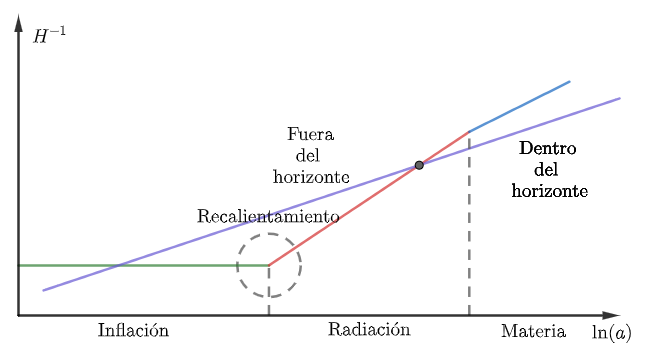
\includegraphics[width=1\linewidth]{Imagenes/Apunte 1/Inflacion.png}
    \caption{esquema de inflación y las escalas}
    \label{fig:inflacion}
\end{figure}

Para que la energía del inflatón se convierta en las partículas que hoy en día tenemos, plantearemos como idea que el inflatón haya estado acoplado con los distintos campos que dan lugar a las partículas tal que luego el inflatón decaiga en estas partículas. A la etapa del Universo en que se producen partículas mediante efectos no perturbativos, se la conoce como \textit{preheating}.

\subsubsection{Parametric resonance of Bosons.}

Si el potencial del inflatón tiene una forma monomial $(\displaystyle \alpha \phi^p)$ durante las etapas tardías de la inflación, el campo empezará a oscilar alrededor del mínimo de este potencial. Típicamente ésto se hará con amplitudes grandes.

Las oscilaciones de este potencial pueden inducir resonancias paramétricas en las partículas con las que se encuentra acoplado el campo del inflatón, ésto dependerá de qué tan fuerte es el acople entre los campos. De este modo, esta resonancia permite la creación de partículas bosónicas. Gracias a ésto, la transferencia de energía es exponencialmente rápida y termina luego de pocas oscilaciones del campo.

En el caso de los fermiones, el principio de exclusión de Pauli bloquea la posibilidad de que la resonancia se desarrolle. Sin embargo, parte de la transferencia de la energía del inflatón se transmite a las especies fermiónicas con longitudes de onda más cortas que las oscilaciones del inflatón.

La resonancia paramétrica de bosones se esperan que generen ondas gravitacionales. Para ver ésto, pensemos que el inflatón se encuentra inicialmente oscilando homogéneamente alrededor del mínimo del potencial con un término del potencial de acople con el campo bosónico $X$ (campo hijo) que es de la forma $g^2 X^2 \phi^2$, siendo la ecuación de movimiento de la forma

\begin{equation}
    \begin{cases}
        \displaystyle \ddot{\phi} - \frac{1}{a^2} \nabla^2 \phi + 3 H \dot{\phi} + g^2 X^2 \phi + \frac{\partial V}{\partial \phi} &= 0\\
        \displaystyle \ddot{X} - \frac{1}{a^2} \nabla^2 X + 3 H \dot{X} + g^2 X \phi^2 &= 0
    \end{cases}
\end{equation}

\noindent
asumiendo que $\phi$ es homogéneo $(\nabla^2 \phi = 0)$ y que es despreciable el \textit{feedback} entre el campo hijo y el inflatón inicialmente, entonces podemos ver que la primera ecuación para un potencial monomial $V (\phi) \propto V^n$ admite una solución oscilatoria de la forma $\phi (t) = \Phi (t) \ F(t)$ dónde $\Phi (t) = \displaystyle \Phi_i \left( \frac{t}{t_i} \right)^{\displaystyle - \frac{2}{n}}$. 

Para potenciales monomiales de la forma $\displaystyle V(\phi) = \frac{\lambda}{n} M^{4 - n} \phi^n$ con $M$ un factor de masa y $\lambda$ un parámetro adimensional, la función $F(t)$ no es periódica salvo para $n = 2$. Y la frecuencia de oscilación cambia como $\Omega_{osc} = \displaystyle \sqrt{\frac{d^2 V}{d\phi^2}} = \sqrt{\lambda} M \left( \frac{\Phi}{M} \right)^{\displaystyle \frac{n}{2} - 1}$.

En el universo temprano serán los momentos dónde será más relevante la resonancia paramétrica, en éste tenemos que el campo del inflatón será clásico y homogéneo mientras que el campo hijo $X$ será considerado como cuántico e inicialmente en vacío. Entonces, como el campo $X$ es cuántico podemos hacer la descomposición estándar

\begin{equation}
    X (\textbf{x}, t) = \frac{1}{(2 \pi)^3 \ a(t)} \int e^{- i \textbf{k} \textbf{x}} \left[ \hat{a}_\textbf{k} \chi_\textbf{k} (t) + \hat{a}_{- \textbf{k}}^\dagger \chi^*_{-\textbf{k}} (t) \right] \ d \textbf{k}
\end{equation}

\noindent
dónde las relaciones de conmutación son las usuales $\displaystyle \left[ \hat{a}_{\textbf{k}}, \hat{a}_{\textbf{k}^\prime}^\dagger \right] = (2\pi)^3 \ \delta (\textbf{k} - \textbf{k}^\prime)$ con $\hat{a}_\textbf{k} \ket{0} = 0$. Podemos también redefinir las variables de campo como

\begin{equation}
    \varphi \equiv a(t) \ \frac{\phi}{\Phi_i} \hspace{2cm} \chi \equiv a(t) \ X
\end{equation}

\noindent
de modo tal que la ecuación de movimiento del campo hijo es

\begin{equation}
    \frac{d^2 \chi_k}{dz^2} + \left( \kappa^2 + q_i \varphi^2 \right) \chi_k \simeq 0
\end{equation}

\noindent
dónde 

\begin{equation}
    \kappa = \frac{k}{\omega_i}, \hspace{1cm} q_i = \frac{g^2 \Phi_i^2}{\omega^2_i}, \hspace{1cm} z = \omega_i \int \frac{dt^\prime}{a(t^\prime)}, \hspace{1cm} \omega_i = \sqrt{\lambda} M \left( \frac{\Phi_i}{M} \right)^{\displaystyle \frac{n}{2} - 1}
\end{equation}

\noindent
a $q_i$ lo conocemos como el parámetro de resonancia. Y dado un parámetro de resonancia, tendremos bandas de resonancia dónde las amplitudes de los modos del campo dentro de esa banda crecen exponencialmente. Entonces, como consecuencia del carácter oscilatorio del inflatón tenemos que $\chi_k \sim e^{\mu_q (\kappa) z}$ dónde $\mu_q (\kappa)$ es una función compleja conocida como \textit{índice Floquet}. Este comportamiento inestable es el que se conoce como resonancia paramétrica y este crecimiento exponencial en los modos de $\chi_k$ es lo que se interpreta como la creación abrupta de partículas y lo podemos ver a partir de ver el número de ocupación de los modos inestables: $\displaystyle n_k \propto |\chi_k|^2 \sim e^{2 \mu_q (\kappa) z}$, también esto implica que se desarrollan inhomogeneidades que no dependen del tiempo y que se convertirán en fuentes de ondas gravitatorias.

La densidad de energía para el espectro del fondo estocástico de ondas en las escalas subhorizonte se puede expresar como

\begin{equation}
    \frac{d \rho_{GW}}{d \ln k} (k, \tau) = \frac{2}{\pi} \frac{G k^3}{a^4 (\tau)} \int_{\tau_i}^\tau a(\tau^\prime) \ a(\tau^{\prime\prime}) \cos \left[ k \left( \tau^\prime - \tau^{\prime\prime} \right) \right] \Pi^2 \left( k, \tau^\prime, \tau^{\prime\prime} \right) \ d\tau^\prime \ d\tau^{\prime\prime}
\end{equation}

\noindent
dónde se define

\begin{equation}
    \bra{0} \Pi_{ij}^{TT} (\textbf{k}, \tau) \ \Pi_{ij}^{TT*} (\textbf{k}^\prime, \tau^\prime) \ket{0} \equiv (2 \pi)^3 \Pi^2 (k, \tau, \tau^\prime) \ \delta^{(3)} (\textbf{k} - \textbf{k}^\prime)
\end{equation}

\noindent
y el tensor de perturbación del tensor de energía momento va a ser en nuestro caso $\displaystyle \Pi_{ij}^{TT} = \frac{1}{a^2} \left\{ \partial_i \chi \partial_j \chi \right\}^{TT}$, entonces nos queda que la amplitud $\Pi^2 (k, \tau, \tau^\prime)$ la podemos encontrar como

\begin{equation}
    \Pi^2 (k, \tau, \tau^\prime) = \int \frac{p^6 \sin^5 \theta}{4 \pi^2 a^2 (\tau) \ a^2 (\tau^\prime)} \chi_\textbf{p} (\tau) \ \chi_{\textbf{k} - \textbf{p}} (\tau) \ \chi_{\textbf{k} - \textbf{p}}^* (\tau^\prime) \ \chi^*_\textbf{p} (\tau^\prime) \ dp \ d\theta
\end{equation}

\noindent
metiendolo en la densidad de energía tenemos

\begin{equation}
    \frac{d \rho_{GW}}{d \ln k} (k, t) = \frac{G k^3}{2 \pi^3} \int p^6 \sin^5 \theta \left( \left| I_{(c)} (k, p, \theta, \tau) \right|^2 + \left| I_{(s)} (k, p, \theta, \tau) \right|^2 \right) \ dp \ d\theta
\end{equation}

\noindent
dónde 

\begin{equation}
    I_{(c)} \equiv \int_{\tau_i}^\tau \cos (k \tau^\prime) \ \chi_{\textbf{k} - \textbf{p}} (\tau^\prime) \ \chi_\textbf{p} (\tau^\prime) \frac{d\tau^\prime}{a(\tau^\prime)} \hspace{1cm} I_{(s)} \equiv \int_{\tau_i}^\tau \sin (k \tau^\prime) \ \chi_{\textbf{k} - \textbf{p}} (\tau^\prime) \ \chi_\textbf{p} (\tau^\prime) \frac{d\tau^\prime}{a(\tau^\prime)}
\end{equation}

El espectro de las ondas gravitatorias tiene un pico bien definido a la escala determinada por el parámetro de resonancia. Cuando tenemos $q_i > 1$ tenemos lo que se conoce como resonancia amplia, y es el régimen en el cual las amplitudes dentro de una esfera de Bose crecen exponencialmente, pero las que están afuera no producen ondas gravitacionales. Dentro de la esfera están todos los modos con $\kappa \leq \kappa_* \sim \sqrt[4]{q_i}$. El pico de amplitud para las ondas gravitacionales a tiempo $t = t_f$ está dado por la forma

\begin{equation}
    \Omega_{GW}^{(f)} (\kappa_p) \simeq \frac{C^2}{8 \pi^4} \frac{\omega_i^6}{\rho_i m_{p}^2} q_i^{\displaystyle - \frac{1}{2} + \delta}
\end{equation}

\noindent
dónde $\displaystyle \delta = \frac{d \ln \Omega_{GW}}{d \ln q_i} + \frac{1}{2}$ que cuantifica la desviación como consecuencia de las no linealidades con respecto al escaleo de la forma $\Omega_{GW} \propto q_i^{ - 1/2}$, y $C$ es una constante adimensional que caracteriza la amplitud de las fluctuaciones del campo dentro de la esfera de Bose, y la podemos calcular como 

\begin{equation}
    k_* \left| X_k^{(c)} \right|^2 = C q_i^{-1} \ \theta (k_* - k)
\end{equation}

Las ondas gravitatorias inicialmente son creadas en un régimen lineal, dónde exponencialmente las fluctuaciones del campo inflatón crece. A medida que crecen estas perturbaciones, la energía del inflatón se transfiere al campo hijo hasta que la resonancia llega al final cuando se transfirió suficiente energía. A lo largo de este proceso, el sistema si convierte no lineal generando ondas gravitacionales hasta que los campos se relajen llegando a un régimen estacionario dónde la generación de ondas gravitacionales se termina.

\paragraph{Anisotropies in the gravitational wave background}